% =============================================================================
%  LATEX COMPLETE REFERENCE — A Learning Project
%  Compile with: pdflatex main.tex (twice for references)
%  Or: xelatex main.tex
% =============================================================================

% --- PREAMBLE: Everything before \begin{document} ---
\documentclass[12pt, a4paper]{report}

% ========================== PACKAGES ==========================================
% Packages extend LaTeX beyond its core. Load them in the preamble, after
% \documentclass but before \begin{document}. Order matters for some packages.

% -- Encoding & fonts --
\usepackage[utf8]{inputenc}          % Allow UTF-8 characters (accented letters etc.)
\usepackage[T1]{fontenc}             % Use 8-bit font encoding for proper hyphenation

% -- Page layout --
\usepackage{geometry}                % Control margins, paper size, orientation

% -- Graphics & drawing --
\usepackage{graphicx}                % \includegraphics — insert PNG, PDF, JPG images
\usepackage{tikz}                    % Programmable vector graphics inside LaTeX
\usetikzlibrary{shapes.geometric, positioning, arrows.meta}
                                     % TikZ libraries: extra shapes, relative positioning, arrow heads
\usepackage{pgfplots}                % Publication-quality 2D/3D plots built on TikZ
\pgfplotsset{compat=1.18}           % Pin pgfplots API version to avoid deprecation warnings

% -- Mathematics --
\usepackage{amsmath, amssymb, amsthm} % amsmath: align, cases, matrices; amssymb: extra symbols; amsthm: theorem environments

% -- Tables --
\usepackage{booktabs}                % \toprule/\midrule/\bottomrule — professional horizontal rules
\usepackage{array}                   % Extends column types (m{}, >{}, p{})
\usepackage{longtable}               % Tables that break across pages
\usepackage{multirow}                % \multirow — cells spanning multiple rows
\usepackage{tabularx}                % Auto-wrapping X column for fixed-width tables

% -- Floats & captions --
\usepackage{float}                   % [H] placement — force float exactly here
\usepackage{caption}                 % Fine-tune caption fonts, labels, spacing
\usepackage{subcaption}              % Subfigures / subtables inside a figure

% -- Text & formatting --
\usepackage[table]{xcolor}           % \textcolor, \colorbox, \rowcolor; [table] adds table coloring support
\usepackage{enumitem}                % Custom list labels, spacing, numbering start
\usepackage{parskip}                 % Remove paragraph indent, add vertical skip instead
\usepackage{indentfirst}             % Indent the very first paragraph after a heading

% -- Code listings --
\usepackage{listings}                % Syntax-highlighted code blocks (see \lstset below)
\usepackage{fancyvrb}                % Enhanced verbatim with frames, font control

% -- Cross-references & links --
\usepackage{hyperref}                % Clickable refs, \url, \href — load late in preamble
\usepackage{url}                     % Line-breakable URLs in text

% -- Structure --
\usepackage{fancyhdr}                % Custom headers (\fancyhead) and footers (\fancyfoot)
\usepackage{tocloft}                 % Style the table of contents, list of figures/tables
\usepackage{titlesec}                % Customize chapter/section title formatting
\usepackage{appendix}                % \appendix + clearer appendix numbering

% -- Science --
\usepackage{siunitx}                 % Proper SI units: \SI{9.8}{m/s^2}

% ========================== PAGE LAYOUT =======================================
\geometry{
    left=2.5cm,
    right=2.5cm,
    top=2.5cm,
    bottom=2.5cm,
    headheight=14.5pt                % Must be >= actual header height to avoid fancyhdr warning
}

% ========================== HEADER / FOOTER ===================================
\pagestyle{fancy}
\fancyhf{}                           % Clear defaults
\fancyhead[L]{\leftmark}             % Left header = chapter name
\fancyhead[R]{\thepage}              % Right header = page number
\fancyfoot[C]{\textit{LaTeX Complete Reference}} % Center footer
\renewcommand{\headrulewidth}{0.4pt}
\renewcommand{\footrulewidth}{0.4pt}

% ========================== HYPERREF CONFIG ===================================
\hypersetup{
    colorlinks=true,
    linkcolor=blue!70!black,
    filecolor=magenta,
    urlcolor=cyan!60!black,
    citecolor=green!50!black,
    pdftitle={LaTeX Complete Reference},
    pdfauthor={Learner},
    pdfsubject={LaTeX Tutorial},
}

% ========================== CODE LISTING STYLE ================================
% Global defaults for every \begin{lstlisting} block.  Override per-block with
% [language=Python, caption={…}] etc.

\lstset{
    basicstyle=\ttfamily\small,                  % Monospace font, slightly smaller than body
    keywordstyle=\color{blue}\bfseries,          % Language keywords (def, for, if …)
    commentstyle=\color{green!50!black}\itshape, % Comments — dark green italic
    stringstyle=\color{red!70!black},            % String literals — dark red
    numbers=left,                                % Line numbers on the left gutter
    numberstyle=\tiny\color{gray},               % Line-number font
    frame=single,                                % Thin border around each listing
    breaklines=true,                             % Wrap long lines automatically
    captionpos=b,                                % Caption rendered below the listing
    tabsize=4,                                   % Tab width in spaces
    showstringspaces=false,                      % Don't mark spaces inside strings
}

% ========================== CUSTOM COLORS =====================================
\definecolor{myblue}{RGB}{0, 102, 204}
\definecolor{mygray}{RGB}{128, 128, 128}
\definecolor{mygreen}{RGB}{0, 128, 0}

% ========================== CUSTOM COMMANDS ===================================
% Define project-wide shorthand commands here.
% See Chapter 14 for how to create your own commands and environments.

\newcommand{\latex}{\LaTeX}                     % Shorthand: \latex → LaTeX logo
\newcommand{\important}[1]{\textbf{\color{red}#1}}  % Red bold callout for critical warnings
\newcommand{\note}[1]{\textit{Note: #1}}              % Italic "Note: …" for tips
\newenvironment{demoobox}[1]
    {\begin{center}\fbox{\begin{minipage}{0.9\textwidth}\textbf{#1}\par\smallskip}}
    {\end{minipage}\end{center}}                       % Demo box for ch14

% ========================== TITLE INFO ========================================
\title{
    \vspace{-2cm}
    \includegraphics[width=0.3\textwidth]{example-image-a}\\[1cm]
    {\Huge \bfseries \LaTeX{} Complete Reference}\\[0.5cm]
    {\Large A Comprehensive Learning Guide}
}
\author{New Learner}
\date{\today}

% =============================================================================
%  DOCUMENT BEGINS
% =============================================================================
\begin{document}

% --- Title Page ---
\maketitle
\thispagestyle{empty}

% --- Table of Contents ---
\newpage
\tableofcontents
\newpage

% =============================================================================
%  CHAPTER 1: Document Structure & Document Classes
% =============================================================================
% =============================================================================
%  CHAPTER 1: Document Structure & Document Classes
% =============================================================================

\chapter{Document Structure \& Document Classes}

Every \latex{} document consists of two main parts:
\begin{enumerate}
    \item \textbf{Preamble} — everything before \verb|\begin{document}|
    \item \textbf{Body} — the content between \verb|\begin{document}| and \verb|\end{document}|
\end{enumerate}

% ------------------------------------------------------------------
\section{Document Classes}
\label{sec:docclasses}

The \verb|\documentclass| command must be the very first command. It defines the type of document.

\begin{table}[H]
\centering
\begin{tabular}{lll}
\toprule
\textbf{Class} & \textbf{Purpose} & \textbf{Sectioning} \\
\midrule
\texttt{article} & Short documents, journal papers & section, subsection \\
\texttt{report}  & Longer documents, theses        & chapter, section \\
\texttt{book}    & Full books                      & part, chapter, section \\
\texttt{letter}  & Letters                         & — \\
\texttt{beamer}  & Presentations/slides            & frame \\
\texttt{scrartcl} & KOMA-Script article            & section \\
\texttt{scrreprt} & KOMA-Script report             & chapter \\
\texttt{scrbook}  & KOMA-Script book               & part, chapter \\
\bottomrule
\end{tabular}
\caption{Common document classes in \latex{}}
\end{table}

\subsection{Document Class Options}

Class options go in square brackets: \verb|\documentclass[options]{class}|

\begin{table}[H]
\centering
\begin{tabular}{ll}
\toprule
\textbf{Option} & \textbf{Effect} \\
\midrule
\texttt{12pt}        & Sets font size (10pt, 11pt, 12pt) \\
\texttt{a4paper}     & Sets paper size (a4paper, letterpaper, legalpaper) \\
\texttt{twoside}     & Formats for two-sided printing \\
\texttt{oneside}     & Formats for one-sided printing (default) \\
\texttt{landscape}   & Landscape orientation \\
\texttt{draft}       & Draft mode — marks overfull boxes \\
\texttt{final}       & Final mode (default) \\
\texttt{twocolumn}   & Two-column layout \\
\texttt{titlepage}   & Title on a separate page \\
\texttt{openright}   & Chapters start on right-hand page \\
\texttt{leqno}       & Equation numbers on left \\
\texttt{fleqn}       & Left-aligned equations \\
\bottomrule
\end{tabular}
\caption{Common document class options}
\end{table}

\begin{lstlisting}[language={[LaTeX]TeX}, caption=Basic document structure]
\documentclass[12pt, a4paper]{article}

% === PREAMBLE ===
% Load packages, define commands, set options here
\usepackage[utf8]{inputenc}
\usepackage{graphicx}
\title{My First Document}
\author{Author Name}

% === BODY ===
\begin{document}
\maketitle
Hello, World!
\end{document}
\end{lstlisting}

% ------------------------------------------------------------------
\section{Sectioning Commands}

\latex{} provides a hierarchy of sectioning commands:

\begin{lstlisting}[language={[LaTeX]TeX}, caption=Sectioning hierarchy]
\part{Part Title}          % Level -1 (book/report only)
\chapter{Chapter Title}    % Level 0  (book/report only)
\section{Section Title}    % Level 1
\subsection{Subsection}    % Level 2
\subsubsection{Sub-sub}    % Level 3
\paragraph{Paragraph}      % Level 4
\subparagraph{Subparagraph}% Level 5
\end{lstlisting}

\subsection{Starred Versions}

Each sectioning command has a starred version (e.g., \verb|\section*{Title}|) that:
\begin{itemize}
    \item Does \emph{not} add a number
    \item Does \emph{not} appear in the table of contents
\end{itemize}

% ------------------------------------------------------------------
\section{Input and Include}

Split large documents into multiple files:

\begin{lstlisting}[language={[LaTeX]TeX}, caption=File inclusion commands]
% \input{file}     -- inserts file content inline (no page break)
% \include{file}   -- inserts file with \clearpage before and after
%                    (cannot be nested)

\input{chapters/chapter1}     % Preferred for small files
\include{chapters/chapter2}   % Preferred for chapters
\end{lstlisting}

\begin{table}[H]
\centering
\begin{tabular}{lcc}
\toprule
\textbf{Feature} & \textbf{\texttt{\textbackslash input}} & \textbf{\texttt{\textbackslash include}} \\
\midrule
Page breaks    & No  & Yes \\
Can be nested  & Yes & No  \\
Selective compilation & No & Yes (\texttt{\textbackslash includeonly}) \\
\bottomrule
\end{tabular}
\caption{Comparison of \texttt{\textbackslash input} vs \texttt{\textbackslash include}}
\end{table}

% ------------------------------------------------------------------
\section{Comments}

\begin{lstlisting}[language={[LaTeX]TeX}, caption=Comments in LaTeX]
% This is a single-line comment.
% Everything after % on the line is ignored.

% For multi-line comments, use the verbatim package:
\usepackage{verbatim}
\begin{comment}
This entire block is commented out.
Line two of the comment.
Line three.
\end{comment}
\end{lstlisting}

% ------------------------------------------------------------------
\section{Special Characters}

The following characters are \important{reserved} in \latex{} and need special handling:

\begin{table}[H]
\centering
\begin{tabular}{cll}
\toprule
\textbf{Character} & \textbf{Purpose} & \textbf{To Print It} \\
\midrule
\texttt{\#}  & Macro parameter      & \verb|\#| \\
\texttt{\$}  & Math mode            & \verb|\$| \\
\texttt{\%}  & Comment              & \verb|\%| \\
\texttt{\&}  & Table column sep.    & \verb|\&| \\
\texttt{\_}  & Subscript (math)     & \verb|\_| \\
\texttt{\{}  & Group begin          & \verb|\{| \\
\texttt{\}}  & Group end            & \verb|\}| \\
\texttt{\~{}}& Non-breaking space   & \verb|\~{}| or \verb|\textasciitilde| \\
\texttt{\^{}}& Circumflex accent    & \verb|\^{}| or \verb|\textasciicircum| \\
\texttt{\textbackslash} & Command prefix & \verb|\textbackslash| \\
\bottomrule
\end{tabular}
\caption{Special characters in \latex{}}
\end{table}

\note{Accented characters can be typed directly in UTF-8: é, ü, ñ, ç, etc.}


% =============================================================================
%  CHAPTER 2: Text Formatting & Fonts
% =============================================================================
% =============================================================================
%  CHAPTER 2: Text Formatting & Fonts
% =============================================================================

\chapter{Text Formatting \& Fonts}

\section{Font Styles}

\latex{} provides command pairs for font switching — one with \emph{declaration syntax} (affects all following text) and one with \emph{command syntax} (takes an argument).

\begin{table}[H]
\centering
\begin{tabular}{lll}
\toprule
\textbf{Style} & \textbf{Declaration} & \textbf{Command} \\
\midrule
\textbf{Bold}          & \verb|\bfseries|  & \verb|\textbf{...}| \\
\textit{Italic}        & \verb|\itshape|   & \verb|\textit{...}| \\
\textsl{Slanted}       & \verb|\slshape|   & \verb|\textsl{...}| \\
\texttt{Monospace}     & \verb|\ttfamily|  & \verb|\texttt{...}| \\
\textsf{Sans-serif}    & \verb|\sffamily|  & \verb|\textsf{...}| \\
\textsc{Small Caps}    & \verb|\scshape|   & \verb|\textsc{...}| \\
\textmd{Medium}        & \verb|\mdseries|  & \verb|\textmd{...}| \\
Upright                & \verb|\upshape|   & \verb|\textup{...}| \\
\bottomrule
\end{tabular}
\caption{Font style commands}
\end{table}

\subsection{Examples}

\begin{itemize}
    \item \textbf{Bold text} with \verb|\textbf{Bold text}|
    \item \textit{Italic text} with \verb|\textit{Italic text}|
    \item \texttt{Typewriter text} with \verb|\texttt{Typewriter text}|
    \item \textsf{Sans-serif text} with \verb|\textsf{Sans-serif text}|
    \item \textsc{Small Capitals} with \verb|\textsc{Small Capitals}|
    \item \textsl{Slanted text} with \verb|\textsl{Slanted text}|
    \item \emph{Emphasized text} — \verb|\emph{}| toggles italic inside roman and roman inside italic
    \item \emph{This is \emph{nested} emphasis} — \verb|\emph{This is \emph{nested} emphasis}|
\end{itemize}

% ------------------------------------------------------------------
\section{Font Sizes}

Size commands are \emph{declarations} — they affect everything until the end of the group:

\begin{table}[H]
\centering
\begin{tabular}{ll}
\toprule
\textbf{Command} & \textbf{Result} \\
\midrule
\verb|\tiny|         & {\tiny Sample text} \\
\verb|\scriptsize|   & {\scriptsize Sample text} \\
\verb|\footnotesize| & {\footnotesize Sample text} \\
\verb|\small|        & {\small Sample text} \\
\verb|\normalsize|   & {\normalsize Sample text} \\
\verb|\large|        & {\large Sample text} \\
\verb|\Large|        & {\Large Sample text} \\
\verb|\LARGE|        & {\LARGE Sample text} \\
\verb|\huge|         & {\huge Sample text} \\
\verb|\Huge|         & {\Huge Sample text} \\
\bottomrule
\end{tabular}
\caption{Font size commands (relative to base document font size)}
\end{table}

\begin{lstlisting}[language={[LaTeX]TeX}, caption=Font size usage]
{\large This text is large.}
{\Large\bfseries This text is large and bold.}
\end{lstlisting}

% ------------------------------------------------------------------
\section{Text Alignment}

\subsection{Centering}

\begin{lstlisting}[language={[LaTeX]TeX}, caption=Centering text]
% Environment form:
\begin{center}
    This text is centered.
\end{center}

% Declaration form (affects rest of group):
{\centering This text is centered.\par}
\end{lstlisting}

\begin{center}
    This is centered text using the \texttt{center} environment.
\end{center}

\subsection{Flush Left (Ragged Right)}

\begin{lstlisting}[language={[LaTeX]TeX}, caption=Left-aligned text]
\begin{flushleft}
    This text is left-aligned.
\end{flushleft}
\end{lstlisting}

\subsection{Flush Right (Ragged Left)}

\begin{lstlisting}[language={[LaTeX]TeX}, caption=Right-aligned text]
\begin{flushright}
    This text is right-aligned.
\end{flushright}
\end{lstlisting}

\begin{flushright}
    This is right-aligned text.
\end{flushright}

% ------------------------------------------------------------------
\section{Line \& Paragraph Spacing}

\begin{lstlisting}[language={[LaTeX]TeX}, caption=Line spacing]
% Single spacing (default)
% Double spacing:
\usepackage{setspace}
\doublespacing

% 1.5 spacing:
\onehalfspacing

% Custom spacing:
\setstretch{1.25}

% Line break (new line, same paragraph):
Line one.\\
Line two.

% Line break with extra space:
Line one.\\[12pt]
Line two with 12pt gap above.

% New paragraph (blank line in source):
Paragraph one.

Paragraph two.

% Horizontal spacing:
Word\hspace{1cm}Word          % 1cm horizontal space
Word\hspace{\fill}Word        % Stretchy space (pushes to margins)
Word\hfill Word               % Shorthand for \hspace{\fill}
\end{lstlisting}

\subsection{Vertical Spacing}

\begin{lstlisting}[language={[LaTeX]TeX}, caption=Vertical spacing]
\vspace{1cm}          % 1cm vertical space
\vspace*{1cm}         % Forced space (even at page top)
\vspace{\fill}        % Stretchy vertical space
\vfill                % Shorthand for \vspace{\fill}
\bigskip              % Large vertical skip (~12pt)
\medskip              % Medium vertical skip (~6pt)
\smallskip            % Small vertical skip (~3pt)
\end{lstlisting}

\subsection{Horizontal Spacing}

\begin{table}[H]
\centering
\begin{tabular}{lll}
\toprule
\textbf{Command} & \textbf{Width} & \textbf{Description} \\
\midrule
\verb|\,|    or \verb|\thinspace|   & $\sim$3/18 quad & Thin space \\
\verb|\:|    or \verb|\medspace|    & $\sim$4/18 quad & Medium space \\
\verb|\;|    or \verb|\thickspace|  & $\sim$5/18 quad & Thick space \\
\verb|\!|                          & $-$3/18 quad    & Negative thin space \\
\verb|\enspace|                     & 0.5em           & En-space \\
\verb|\quad|                        & 1em             & Quad space \\
\verb|\qquad|                       & 2em             & Double quad \\
\verb|\~{}|                         & variable        & Non-breaking space \\
\verb|\hspace{length}|              & variable        & Custom horizontal space \\
\bottomrule
\end{tabular}
\caption{Horizontal spacing commands}
\end{table}

% ------------------------------------------------------------------
\section{Text Decoration \& Color}

\subsection{Underline and Overline}

\begin{lstlisting}[language={[LaTeX]TeX}, caption=Underline and overline]
\underline{Underlined text}
\overline{Overlined text}        % Works in math mode too
\end{lstlisting}

\underline{Underlined text example.}

\subsection{Strikethrough (requires ulem package)}

\begin{lstlisting}[language={[LaTeX]TeX}, caption=Strikethrough]
\usepackage[normalem]{ulem}

\sout{Strikethrough text}
\uwave{Wavy underline}
\xout{Crossed out with /}
\end{lstlisting}

\subsection{Text Color (xcolor package)}

\begin{lstlisting}[language={[LaTeX]TeX}, caption=Using colors]
\textcolor{red}{Red text}
\textcolor{blue}{Blue text}
\textcolor{green!50!black}{Dark green text}

% Color as declaration:
{\color{red} This entire block is red.}

% Define custom colors:
\definecolor{mycolor}{RGB}{102, 178, 255}
\textcolor{mycolor}{Custom colored text}

% Background color (requires xcolor with table option):
\colorbox{yellow}{Highlighted text}
\fcolorbox{red}{yellow}{Box with red border and yellow background}
\end{lstlisting}

Examples: \textcolor{red}{Red}, \textcolor{blue}{Blue}, \textcolor{green!50!black}{Dark Green}, \colorbox{yellow}{Highlighted}

% ------------------------------------------------------------------
\section{Accents and Special Characters}

\begin{table}[H]
\centering
\begin{tabular}{llll}
\toprule
\textbf{Accent} & \textbf{Command} & \textbf{Result} & \textbf{Alt (UTF-8)} \\
\midrule
Grave        & \verb|\`{o}| & \`{o} & \`o \\
Acute        & \verb|\'{o}| & \'{o} & \'o \\
Circumflex   & \verb|\^{o}| & \^{o} & \^o \\
Tilde        & \verb|\~{o}| & \~{o} & \~o \\
Umlaut       & \verb|\"{o}| & \"{o} & \"o \\
Cedilla      & \verb|\c{c}| & \c{c} & \c{c} \\
Ogonek       & \verb|\k{a}| & \k{a} & \\
Macron       & \verb|\={o}| & \={o} & \\
Breve        & \verb|\u{o}| & \u{o} & \\
Dot          & \verb|\.{o}| & \.{o} & \\
Ring         & \verb|\r{a}| & \r{a} & \\
Hacek        & \verb|\v{o}| & \v{o} & \\
Double acute & \verb|\H{o}| & \H{o} & \\
\bottomrule
\end{tabular}
\caption{Accent commands}
\end{table}

% ------------------------------------------------------------------
\section{Dashes and Quotes}

\begin{table}[H]
\centering
\begin{tabular}{llll}
\toprule
\textbf{Type} & \textbf{Source} & \textbf{Result} & \textbf{Usage} \\
\midrule
Hyphen    & \verb|-|   & mother-in-law & Compound words \\
En-dash   & \verb|--|  & pages 1--10   & Ranges \\
Em-dash   & \verb|---| & Yes---indeed   & Interruptions \\
Minus     & \verb|$-$| & $-$           & Mathematical minus \\
\bottomrule
\end{tabular}
\caption{Types of dashes}
\end{table}

\begin{table}[H]
\centering
\begin{tabular}{lll}
\toprule
\textbf{Type} & \textbf{Source} & \textbf{Result} \\
\midrule
Opening double quotes & \verb|``| & ``Hello'' \\
Closing double quotes & \verb|''| & ``Hello'' \\
Opening single quote  & \verb|`|  & `Hello' \\
Closing single quote  & \verb|'|  & `Hello' \\
\bottomrule
\end{tabular}
\caption{Quotation marks}
\end{table}

\note{\latex{} does not use regular keyboard quotes (\texttt{"}). Always use backticks for opening quotes.}


% =============================================================================
%  CHAPTER 3: Lists
% =============================================================================
% =============================================================================
%  CHAPTER 3: Lists
% =============================================================================

\chapter{Lists}

\section{Itemize (Bulleted Lists)}

\begin{lstlisting}[language={[LaTeX]TeX}, caption=Basic itemize list]
\begin{itemize}
    \item First item
    \item Second item
    \item Third item
\end{itemize}
\end{lstlisting}

Result:
\begin{itemize}
    \item First item
    \item Second item
    \item Third item
\end{itemize}

\subsection{Nested Itemize}

\begin{lstlisting}[language={[LaTeX]TeX}, caption=Nested itemize]
\begin{itemize}
    \item First level
    \begin{itemize}
        \item Second level
        \begin{itemize}
            \item Third level
            \begin{itemize}
                \item Fourth level
            \end{itemize}
        \end{itemize}
    \end{itemize}
\end{itemize}
\end{lstlisting}

Result:
\begin{itemize}
    \item First level
    \begin{itemize}
        \item Second level
        \begin{itemize}
            \item Third level
            \begin{itemize}
                \item Fourth level
            \end{itemize}
        \end{itemize}
    \end{itemize}
\end{itemize}

% ------------------------------------------------------------------
\section{Enumerate (Numbered Lists)}

\begin{lstlisting}[language={[LaTeX]TeX}, caption=Basic enumerate list]
\begin{enumerate}
    \item First item
    \item Second item
    \item Third item
\end{enumerate}
\end{lstlisting}

Result:
\begin{enumerate}
    \item First item
    \item Second item
    \item Third item
\end{enumerate}

\subsection{Nested Enumerate}

\begin{enumerate}
    \item First level
    \begin{enumerate}
        \item Second level
        \begin{enumerate}
            \item Third level
            \begin{enumerate}
                \item Fourth level
            \end{enumerate}
        \end{enumerate}
    \end{enumerate}
    \item Back to first level
\end{enumerate}

% ------------------------------------------------------------------
\section{Description Lists}

\begin{lstlisting}[language={[LaTeX]TeX}, caption=Description list]
\begin{description}
    \item[Term 1] Definition or description of term 1.
    \item[Term 2] Definition or description of term 2.
    \item[Term 3] Definition or description of term 3.
\end{description}
\end{lstlisting}

Result:
\begin{description}
    \item[\latex{}] A document preparation system.
    \item[TeX] The typesetting engine by Donald Knuth.
    \item[PDF] Portable Document Format.
\end{description}

% ------------------------------------------------------------------
\section{Customizing Lists with enumitem}

The \texttt{enumitem} package provides powerful list customization.

\subsection{Custom Labels}

\begin{lstlisting}[language={[LaTeX]TeX}, caption=Custom enumerate labels]
% Roman numerals:
\begin{enumerate}[label=\Roman*.]
    \item First
    \item Second
\end{enumerate}

% Alphabetical:
\begin{enumerate}[label=\alph*)]
    \item First
    \item Second
\end{enumerate}

% Custom format:
\begin{enumerate}[label=Step \arabic*:)]
    \item First
    \item Second
\end{enumerate}
\end{lstlisting}

Roman numerals:
\begin{enumerate}[label=\Roman*.]
    \item First
    \item Second
    \item Third
\end{enumerate}

Alphabetical:
\begin{enumerate}[label=\alph*)]
    \item First
    \item Second
    \item Third
\end{enumerate}

Custom format:
\begin{enumerate}[label=Step \arabic*:]
    \item Gather requirements
    \item Design solution
    \item Implement
    \item Test
\end{enumerate}

\subsection{Custom Bullet Symbols}

\begin{lstlisting}[language={[LaTeX]TeX}, caption=Custom bullets]
\begin{itemize}[label=$\star$]
    \item Star bullet
    \item Another star
\end{itemize}

\begin{itemize}[label=\textbullet]
    \item Standard bullet
\end{itemize}

\begin{itemize}[label=$\checkmark$]
    \item Checkmark bullet
\end{itemize}
\end{lstlisting}

\begin{itemize}[label=$\star$]
    \item Star bullet one
    \item Star bullet two
\end{itemize}

\begin{itemize}[label=$\checkmark$]
    \item Completed task one
    \item Completed task two
\end{itemize}

\subsection{Spacing Control}

\begin{lstlisting}[language={[LaTeX]TeX}, caption=List spacing]
\begin{itemize}[nosep]           % No extra spacing between items
    \item Compact item 1
    \item Compact item 2
\end{itemize}

\begin{itemize}[topsep=0pt]     % No space above/below list
    \item Item 1
    \item Item 2
\end{itemize}

\begin{enumerate}[start=5]      % Start counting from 5
    \item Fifth
    \item Sixth
\end{enumerate}
\end{lstlisting}

Compact list (\texttt{nosep}):
\begin{itemize}[nosep]
    \item Compact item 1
    \item Compact item 2
    \item Compact item 3
\end{itemize}

Starting from 5:
\begin{enumerate}[start=5]
    \item Fifth
    \item Sixth
    \item Seventh
\end{enumerate}

% ------------------------------------------------------------------
\section{Inline Lists}

\begin{lstlisting}[language={[LaTeX]TeX}, caption=Inline list with enumitem]
\usepackage[inline]{enumitem}

The colors are:
\begin{enumerate*}[label=\arabic*.]
    \item red, \item green, and \item blue.
\end{enumerate*}
\end{lstlisting}

\note{Inline lists require \texttt{\textbackslash usepackage[inline]\{enumitem\}}.}

% ------------------------------------------------------------------
\section{List Summary}

\begin{table}[H]
\centering
\begin{tabular}{llp{6cm}}
\toprule
\textbf{Environment} & \textbf{Best For} & \textbf{Default Label} \\
\midrule
\texttt{itemize}    & Unordered items     & Bullets ($\bullet$, --, *, $\cdot$) \\
\texttt{enumerate}  & Ordered/sequential  & Numbers (1., (a), i., A.) \\
\texttt{description}& Definitions/terms   & Bold label text \\
\bottomrule
\end{tabular}
\caption{List environments summary}
\end{table}


% =============================================================================
%  CHAPTER 4: Tables
% =============================================================================
% =============================================================================
%  CHAPTER 4: Tables
% =============================================================================

\chapter{Tables}

\section{Basic Table (tabular)}

The \texttt{tabular} environment is the fundamental table environment in \latex{}.

\subsection{Column Types}

\begin{table}[H]
\centering
\begin{tabular}{cl}
\toprule
\textbf{Spec} & \textbf{Description} \\
\midrule
\texttt{l} & Left-aligned column \\
\texttt{c} & Centered column \\
\texttt{r} & Right-aligned column \\
\texttt{p\{width\}} & Paragraph column with fixed width \\
\texttt{|} & Vertical line \\
\texttt{@\{text\}} & Replace inter-column space with \textit{text} \\
\bottomrule
\end{tabular}
\caption{Column type specifications}
\end{table}

\subsection{Basic Example}

\begin{lstlisting}[language={[LaTeX]TeX}, caption=Basic tabular]
\begin{tabular}{|l|c|r|}
    \hline
    Left & Center & Right \\
    \hline
    A    & B      & C \\
    \hline
\end{tabular}
\end{lstlisting}

Result:
\begin{tabular}{|l|c|r|}
    \hline
    Left & Center & Right \\
    \hline
    A    & B      & C \\
    \hline
\end{tabular}

% ------------------------------------------------------------------
\section{Table Syntax}

\begin{lstlisting}[language={[LaTeX]TeX}, caption=Table syntax reference]
% &      -- column separator
% \\     -- end of row
% \hline -- horizontal line (spans full width)
% \cline{2-3} -- partial horizontal line (columns 2 to 3)

\begin{tabular}{|l|c|r|}
    \hline
    Name  & Age & Score \\
    \hline
    Alice & 25  & 95 \\
    Bob   & 30  & 87 \\
    \cline{2-3}
    \multicolumn{1}{c|}{} & \multicolumn{2}{c}{Partial line} \\
    \hline
\end{tabular}
\end{lstlisting}

% ------------------------------------------------------------------
\section{Professional Tables with booktabs}

The \texttt{booktabs} package produces publication-quality tables without vertical lines.

\begin{lstlisting}[language={[LaTeX]TeX}, caption=booktabs example]
\usepackage{booktabs}

\begin{tabular}{lcc}
    \toprule
    Name  & Age & Score \\
    \midrule
    Alice & 25  & 95 \\
    Bob   & 30  & 87 \\
    Carol & 28  & 92 \\
    \bottomrule
\end{tabular}
\end{lstlisting}

Result:
\begin{table}[H]
\centering
\begin{tabular}{lcc}
\toprule
\textbf{Name}  & \textbf{Age} & \textbf{Score} \\
\midrule
Alice & 25  & 95 \\
Bob   & 30  & 87 \\
Carol & 28  & 92 \\
\midrule
\textbf{Average} & \textbf{27.7} & \textbf{91.3} \\
\bottomrule
\end{tabular}
\caption{Student scores using booktabs}
\end{table}

\begin{table}[H]
\centering
\begin{tabular}{ll}
\toprule
\textbf{booktabs command} & \textbf{Purpose} \\
\midrule
\verb|\toprule|    & Top rule (thicker) \\
\verb|\midrule|    & Middle rule (medium) \\
\verb|\bottomrule| & Bottom rule (thicker) \\
\verb|\cmidrule{a-b}| & Partial rule (thinner) \\
\verb|\addlinespace|   & Extra vertical space \\
\bottomrule
\end{tabular}
\caption{booktabs commands}
\end{table}

% ------------------------------------------------------------------
\section{Multi-column and Multi-row}

\subsection{Multi-column (\texttt{\textbackslash multicolumn})}

\begin{lstlisting}[language={[LaTeX]TeX}, caption=Multicolumn]
\multicolumn{number_of_columns}{alignment}{text}
\end{lstlisting}

\begin{table}[H]
\centering
\begin{tabular}{llcc}
\toprule
 & \textbf{Math} & \textbf{Physics} & \textbf{Chemistry} \\
\midrule
Alice  & 95 & 88 & 91 \\
Bob    & 87 & 92 & 85 \\
\midrule
\multicolumn{2}{l}{\textit{Class Average}} & \multicolumn{2}{c}{\textbf{89.7}} \\
\bottomrule
\end{tabular}
\caption{Multicolumn example}
\end{table}

\subsection{Multi-row (multirow package)}

\begin{lstlisting}[language={[LaTeX]TeX}, caption=Multirow]
\usepackage{multirow}
\multirow{number_of_rows}{width}{text}
\end{lstlisting}

\begin{table}[H]
\centering
\begin{tabular}{llcc}
\toprule
\textbf{Category} & \textbf{Subject} & \textbf{Students} & \textbf{Avg Score} \\
\midrule
\multirow{2}{*}{Science} & Physics  & 45 & 88 \\
                          & Chemistry & 38 & 85 \\
\midrule
\multirow{2}{*}{Arts}    & History  & 32 & 91 \\
                          & Literature & 29 & 93 \\
\bottomrule
\end{tabular}
\caption{Multirow example}
\end{table}

% ------------------------------------------------------------------
\section{Fixed-width Tables (tabularx)}

\begin{lstlisting}[language={[LaTeX]TeX}, caption=tabularx]
\usepackage{tabularx}

\begin{tabularx}{\textwidth}{lX}
    \toprule
    Name & Description \\
    \midrule
    Item 1 & This text automatically wraps to fill
             the available column width. \\
    Item 2 & Another long description that wraps
             automatically in the X column. \\
    \bottomrule
\end{tabularx}
\end{lstlisting}

Result:
\begin{table}[H]
\centering
\begin{tabularx}{0.9\textwidth}{lX}
\toprule
\textbf{Command} & \textbf{Description} \\
\midrule
\verb|\LaTeX|   & Produces the \LaTeX{} logo with proper kerning and raised ``A''. \\
\verb|\TeX|     & Produces the \TeX{} logo. \\
\verb|\today|   & Produces the current date. \\
\verb|\tableofcontents| & Generates the table of contents from sectioning commands. \\
\bottomrule
\end{tabularx}
\caption{tabularx with auto-wrapping X column}
\end{table}

% ------------------------------------------------------------------
\section{Multi-page Tables (longtable)}

\begin{lstlisting}[language={[LaTeX]TeX}, caption=longtable]
\usepackage{longtable}

\begin{longtable}{lcc}
    \caption{A long table spanning multiple pages} \\
    \toprule
    Name & Value & Note \\
    \midrule
    \endfirsthead

    \toprule
    Name & Value & Note \\
    \midrule
    \endhead

    \midrule
    \multicolumn{3}{r}{\textit{Continued on next page}} \\
    \endfoot

    \bottomrule
    \endlastfoot

    Data1 & 100 & Note1 \\
    Data2 & 200 & Note2 \\
    % ... many more rows ...
\end{longtable}
\end{lstlisting}

% ------------------------------------------------------------------
\section{Table Placement (Float)}

Tables inside \texttt{table} environment are \emph{floating bodies}:

\begin{lstlisting}[language={[LaTeX]TeX}, caption=Float placement specifiers]
\begin{table}[placement]
    % placement can be:
    % h = here       (approximately at current location)
    % t = top        (top of page)
    % b = bottom     (bottom of page)
    % p = page       (on a separate float page)
    % ! = override   (relax LaTeX's internal rules)
    % H = HERE       (requires float package -- exact placement)
    \centering
    \begin{tabular}{lc}
        ...
    \end{tabular}
    \caption{Table caption}
    \label{tab:mylabel}
\end{table}
\end{lstlisting}

% ------------------------------------------------------------------
\section{Colored Tables}

\begin{lstlisting}[language={[LaTeX]TeX}, caption=Colored table rows]
\usepackage[table]{xcolor}

\rowcolor{gray!20}       % Color entire row
\cellcolor{blue!25}       % Color single cell
\columncolor{green!15}    % Color entire column (in column spec)
\end{lstlisting}

\begin{table}[H]
\centering
\begin{tabular}{lcc}
\toprule
\rowcolor{blue!15}
\textbf{Header 1} & \textbf{Header 2} & \textbf{Header 3} \\
\midrule
Row 1, Col 1 & Row 1, Col 2 & Row 1, Col 3 \\
\rowcolor{gray!10}
Row 2, Col 1 & Row 2, Col 2 & Row 2, Col 3 \\
Row 3, Col 1 & Row 3, Col 2 & Row 3, Col 3 \\
\rowcolor{gray!10}
Row 4, Col 1 & Row 4, Col 2 & Row 4, Col 3 \\
\bottomrule
\end{tabular}
\caption{Alternating row colors}
\end{table}

% ------------------------------------------------------------------
\section{Table Quick Reference}

\begin{table}[H]
\centering
\begin{tabular}{ll}
\toprule
\textbf{Symbol/Command} & \textbf{Meaning} \\
\midrule
\verb|&|               & Column separator \\
\verb|\\|              & Row terminator \\
\verb|\hline|          & Full horizontal line \\
\verb|\cline{a-b}|     & Partial horizontal line \\
\verb|\vline|          & Vertical line (inline) \\
\verb|\multicolumn{n}{spec}{text}| & Span $n$ columns \\
\verb|\multirow{n}{w}{text}| & Span $n$ rows \\
\verb|\toprule|        & booktabs top rule \\
\verb|\midrule|        & booktabs middle rule \\
\verb|\bottomrule|     & booktabs bottom rule \\
\bottomrule
\end{tabular}
\caption{Table syntax quick reference}
\end{table}


% =============================================================================
%  CHAPTER 5: Mathematics
% =============================================================================
% =============================================================================
%  CHAPTER 5: Mathematics
% =============================================================================

\chapter{Mathematics}

\latex{} is renowned for its mathematical typesetting. This chapter covers everything from basic inline formulas to advanced constructs.

% ------------------------------------------------------------------
\section{Math Modes}

There are several ways to enter math mode:

\begin{table}[H]
\centering
\begin{tabular}{lll}
\toprule
\textbf{Type} & \textbf{Syntax} & \textbf{Usage} \\
\midrule
Inline math   & \verb|$...$|            & $E=mc^2$ in text \\
Display math  & \verb|\[...\]|          & Centered, numbered \\
Equation env  & \verb|\begin{equation}| & Centered, numbered \\
Align env     & \verb|\begin{align}|    & Multi-line aligned \\
\bottomrule
\end{tabular}
\caption{Math mode entry points}
\end{table}

\begin{lstlisting}[language={[LaTeX]TeX}, caption=Math modes]
% Inline: the formula flows with text
The energy is $E = mc^2$ according to Einstein.

% Display: the formula is centered on its own line
\[ E = mc^2 \]

% Equation: like display but with a number
\begin{equation}
    E = mc^2 \label{eq:einstein}
\end{equation}

% Starred version: no number
\begin{equation*}
    E = mc^2
\end{equation*}
\end{lstlisting}

% ------------------------------------------------------------------
\section{Superscripts and Subscripts}

\begin{lstlisting}[language={[LaTeX]TeX}, caption=Superscripts and subscripts]
$x^2$              % Superscript: x squared
$x_i$              % Subscript: x sub i
$x_i^2$            % Both: x sub i squared
$x_{i,j}$          % Multi-character subscript: need braces
$a^{b^c}$          % Nested superscript
$2^{10} = 1024$    % Powers
\end{lstlisting}

Results: $x^2$, \quad $x_i$, \quad $x_i^2$, \quad $x_{i,j}$, \quad $a^{b^c}$, \quad $2^{10} = 1024$

% ------------------------------------------------------------------
\section{Fractions}

\begin{lstlisting}[language={[LaTeX]TeX}, caption=Fractions]
$\frac{a}{b}$                          % Basic fraction
$\dfrac{a}{b}$                         % Display-style fraction
$\tfrac{a}{b}$                         % Text-style fraction
$\cfrac{1}{1+\cfrac{1}{2}}$           % Continued fraction
$\binom{n}{k}$                         % Binomial coefficient
\end{lstlisting}

Results: $\frac{a}{b}$, \quad $\dfrac{a}{b}$, \quad $\cfrac{1}{1+\cfrac{1}{2}}$, \quad $\binom{n}{k}$

% ------------------------------------------------------------------
\section{Roots}

\begin{lstlisting}[language={[LaTeX]TeX}, caption=Roots]
$\sqrt{x}$            % Square root
$\sqrt[3]{x}$         % Cube root
$\sqrt[n]{x}$         % nth root
$\sqrt{a^2 + b^2}$    % Complex expression
\end{lstlisting}

Results: $\sqrt{x}$, \quad $\sqrt[3]{x}$, \quad $\sqrt[n]{x}$, \quad $\sqrt{a^2 + b^2}$

% ------------------------------------------------------------------
\section{Sums, Products, Integrals}

\begin{lstlisting}[language={[LaTeX]TeX}, caption=Big operators]
$\sum_{i=1}^{n} x_i$         % Summation
$\prod_{i=1}^{n} x_i$        % Product
$\int_{a}^{b} f(x) dx$       % Definite integral
$\iint_{D} f(x,y) dA$        % Double integral
$\iiint_{V} f(x,y,z) dV$     % Triple integral
$\oint_{C} F \cdot dr$       % Contour integral
$\lim_{x \to \infty} f(x)$  % Limit
$\sup_{x \in S} f(x)$       % Supremum
$\max_{x \in S} f(x)$       % Maximum
$\min_{x \in S} f(x)$       % Minimum
\end{lstlisting}

Display style results:
\[ \sum_{i=1}^{n} x_i \qquad \prod_{i=1}^{n} x_i \qquad \int_{a}^{b} f(x)\,dx \qquad \lim_{x \to \infty} f(x) \]

% ------------------------------------------------------------------
\section{Greek Letters}

\begin{table}[H]
\centering
\begin{tabular}{llll}
\toprule
\textbf{Command} & \textbf{Result} & \textbf{Command} & \textbf{Result} \\
\midrule
\verb|\alpha|     & $\alpha$     & \verb|\Alpha|     & $A$ \\
\verb|\beta|      & $\beta$      & \verb|\gamma|     & $\gamma$ \\
\verb|\delta|     & $\delta$     & \verb|\epsilon|   & $\epsilon$ \\
\verb|\varepsilon|& $\varepsilon$& \verb|\zeta|      & $\zeta$ \\
\verb|\eta|       & $\eta$       & \verb|\theta|     & $\theta$ \\
\verb|\iota|      & $\iota$      & \verb|\kappa|     & $\kappa$ \\
\verb|\lambda|    & $\lambda$    & \verb|\mu|        & $\mu$ \\
\verb|\nu|        & $\nu$        & \verb|\xi|        & $\xi$ \\
\verb|\pi|        & $\pi$        & \verb|\rho|       & $\rho$ \\
\verb|\sigma|     & $\sigma$     & \verb|\tau|       & $\tau$ \\
\verb|\upsilon|   & $\upsilon$   & \verb|\phi|       & $\phi$ \\
\verb|\varphi|    & $\varphi$    & \verb|\chi|       & $\chi$ \\
\verb|\psi|       & $\psi$       & \verb|\omega|     & $\omega$ \\
\midrule
\verb|\Gamma|     & $\Gamma$     & \verb|\Delta|     & $\Delta$ \\
\verb|\Theta|     & $\Theta$     & \verb|\Lambda|    & $\Lambda$ \\
\verb|\Xi|        & $\Xi$        & \verb|\Pi|        & $\Pi$ \\
\verb|\Sigma|     & $\Sigma$     & \verb|\Phi|       & $\Phi$ \\
\verb|\Psi|       & $\Psi$       & \verb|\Omega|     & $\Omega$ \\
\bottomrule
\end{tabular}
\caption{Greek letters}
\end{table}

% ------------------------------------------------------------------
\section{Mathematical Operators and Functions}

\begin{lstlisting}[language={[LaTeX]TeX}, caption=Math operators]
$\sin x$     $\cos x$     $\tan x$
$\arcsin x$  $\arccos x$  $\arctan x$
$\sinh x$    $\cosh x$    $\tanh x$
$\ln x$      $\log x$     $\exp x$
$\det A$     $\dim V$     $\ker f$
$\deg f$     $\gcd(a,b)$  $\hom(A,B)$
$\inf S$     $\sup S$     $\max S$
$\min S$     $\lim f$     $\limsup f$
\end{lstlisting}

% ------------------------------------------------------------------
\section{Relations and Binary Operators}

\begin{table}[H]
\centering
\begin{tabular}{llll}
\toprule
\textbf{Command} & \textbf{Symbol} & \textbf{Command} & \textbf{Symbol} \\
\midrule
\verb|<|      & $<$      & \verb|>|       & $>$ \\
\verb|\leq|   & $\leq$   & \verb|\geq|    & $\geq$ \\
\verb|\neq|   & $\neq$   & \verb|\approx| & $\approx$ \\
\verb|\equiv| & $\equiv$ & \verb|\sim|    & $\sim$ \\
\verb|\propto|& $\propto$& \verb|\ll|     & $\ll$ \\
\verb|\gg|    & $\gg$    & \verb|\in|     & $\in$ \\
\verb|\subset|& $\subset$& \verb|\supset| & $\supset$ \\
\verb|\subseteq| & $\subseteq$ & \verb|\supseteq| & $\supseteq$ \\
\verb|\cup|   & $\cup$   & \verb|\cap|    & $\cap$ \\
\verb|\setminus| & $\setminus$ & \verb|\emptyset| & $\emptyset$ \\
\verb|\pm|    & $\pm$    & \verb|\mp|     & $\mp$ \\
\verb|\times| & $\times$ & \verb|\div|    & $\div$ \\
\verb|\cdot|  & $\cdot$  & \verb|\circ|   & $\circ$ \\
\verb|\otimes|& $\otimes$& \verb|\oplus|  & $\oplus$ \\
\bottomrule
\end{tabular}
\caption{Common mathematical symbols}
\end{table}

% ------------------------------------------------------------------
\section{Arrows}

\begin{table}[H]
\centering
\begin{tabular}{llll}
\toprule
\textbf{Command} & \textbf{Arrow} & \textbf{Command} & \textbf{Arrow} \\
\midrule
\verb|\leftarrow|      & $\leftarrow$      & \verb|\rightarrow|     & $\rightarrow$ \\
\verb|\Leftarrow|      & $\Leftarrow$      & \verb|\Rightarrow|     & $\Rightarrow$ \\
\verb|\leftrightarrow| & $\leftrightarrow$ & \verb|\Leftrightarrow| & $\Leftrightarrow$ \\
\verb|\mapsto|         & $\mapsto$         & \verb|\longmapsto|     & $\longmapsto$ \\
\verb|\uparrow|        & $\uparrow$        & \verb|\downarrow|      & $\downarrow$ \\
\verb|\nearrow|        & $\nearrow$        & \verb|\searrow|        & $\searrow$ \\
\bottomrule
\end{tabular}
\caption{Arrow symbols}
\end{table}

% ------------------------------------------------------------------
\section{Matrices}

The \texttt{amsmath} package provides several matrix environments:

\begin{lstlisting}[language={[LaTeX]TeX}, caption=Matrices]
% Parentheses: ( )
\begin{pmatrix}
    a & b \\
    c & d
\end{pmatrix}

% Brackets: [ ]
\begin{bmatrix}
    a & b \\
    c & d
\end{bmatrix}

% Braces: { }
\begin{Bmatrix}
    a & b \\
    c & d
\end{Bmatrix}

% Vertical bars: | |
\begin{vmatrix}
    a & b \\
    c & d
\end{vmatrix}

% Double vertical bars: || ||
\begin{Vmatrix}
    a & b \\
    c & d
\end{Vmatrix}

% No delimiters
\begin{matrix}
    a & b \\
    c & d
\end{matrix}

% With dots:
\begin{pmatrix}
    a_{11} & a_{12} & \cdots & a_{1n} \\
    a_{21} & a_{22} & \cdots & a_{2n} \\
    \vdots & \vdots & \ddots & \vdots \\
    a_{m1} & a_{m2} & \cdots & a_{mn}
\end{pmatrix}
\end{lstlisting}

Results:
\[
\begin{pmatrix} a & b \\ c & d \end{pmatrix}
\quad
\begin{bmatrix} 1 & 2 \\ 3 & 4 \end{bmatrix}
\quad
\begin{vmatrix} a & b \\ c & d \end{vmatrix}
\]

\[
\begin{pmatrix}
a_{11} & a_{12} & \cdots & a_{1n} \\
a_{21} & a_{22} & \cdots & a_{2n} \\
\vdots & \vdots & \ddots & \vdots \\
a_{m1} & a_{m2} & \cdots & a_{mn}
\end{pmatrix}
\]

% ------------------------------------------------------------------
\section{Multi-line Equations (align)}

\begin{lstlisting}[language={[LaTeX]TeX}, caption=align environment]
\begin{align}
    f(x) &= x^2 + 2x + 1 \\
         &= (x+1)^2 \\
         &= x^2 + 2x + 1 \label{eq:expand}
\end{align}

% align without numbering:
\begin{align*}
    f(x) &= x^2 + 2x + 1 \\
         &= (x+1)^2
\end{align*}

% Number specific lines only:
\begin{align}
    f(x) &= x^2 + 2x + 1 \nonumber \\
         &= (x+1)^2 \\
         &= x^2 + 2x + 1 \nonumber
\end{align}

% Multiple alignment columns:
\begin{align*}
    x &= 1  &  y &= 2  &  z &= 3 \\
    x' &= 4 &  y' &= 5 &  z' &= 6
\end{align*}
\end{lstlisting}

Result:
\begin{align}
    f(x) &= x^2 + 2x + 1 \label{eq:quadratic} \\
         &= (x+1)^2 \nonumber
\end{align}

% ------------------------------------------------------------------
\section{Cases and Piecewise Functions}

\begin{lstlisting}[language={[LaTeX]TeX}, caption=cases environment]
\begin{equation}
    |x| =
    \begin{cases}
        x  & \text{if } x \geq 0 \\
        -x & \text{if } x < 0
    \end{cases}
\end{equation}
\end{lstlisting}

Result:
\begin{equation}
    |x| =
    \begin{cases}
        x  & \text{if } x \geq 0 \\
        -x & \text{if } x < 0
    \end{cases}
\end{equation}

% ------------------------------------------------------------------
\section{Accents in Math Mode}

\begin{table}[H]
\centering
\begin{tabular}{lll}
\toprule
\textbf{Command} & \textbf{Result} & \textbf{Name} \\
\midrule
\verb|\hat{a}|     & $\hat{a}$     & Hat \\
\verb|\bar{a}|     & $\bar{a}$     & Bar \\
\verb|\tilde{a}|   & $\tilde{a}$   & Tilde \\
\verb|\vec{a}|     & $\vec{a}$     & Vector arrow \\
\verb|\dot{a}|     & $\dot{a}$     & Dot \\
\verb|\ddot{a}|    & $\ddot{a}$    & Double dot \\
\verb|\vec{a}|     & $\vec{a}$     & Vector \\
\verb|\widehat{abc}|& $\widehat{abc}$& Wide hat \\
\verb|\widetilde{abc}|& $\widetilde{abc}$& Wide tilde \\
\verb|\overline{abc}| & $\overline{abc}$ & Overline \\
\verb|\underline{abc}| & $\underline{abc}$ & Underline \\
\verb|\overbrace{abc}| & $\overbrace{abc}$ & Overbrace \\
\verb|\underbrace{abc}|& $\underbrace{abc}$& Underbrace \\
\bottomrule
\end{tabular}
\caption{Math accents}
\end{table}

% ------------------------------------------------------------------
\section{Spacing in Math Mode}

\begin{table}[H]
\centering
\begin{tabular}{lll}
\toprule
\textbf{Command} & \textbf{Space} & \textbf{Example} \\
\midrule
\verb|\,|     & Thin space      & $a\,b$ \\
\verb|\:|     & Medium space    & $a\:b$ \\
\verb|\;|     & Thick space     & $a\;b$ \\
\verb|\!|     & Negative thin   & $a\!b$ \\
\verb|\quad|  & 1em space       & $a\quad b$ \\
\verb|\qquad| & 2em space       & $a\qquad b$ \\
\verb|\,|     & & $ab$ (no space for comparison) \\
\bottomrule
\end{tabular}
\caption{Math spacing commands}
\end{table}

% ------------------------------------------------------------------
\section{Text Inside Math Mode}

\begin{lstlisting}[language={[LaTeX]TeX}, caption=Text in math]
$\text{for all } x > 0$           % Regular text in math
$\text{if and only if}$            % Using amsmath \text
$\mathrm{d}x$                      % Upright d for differentials
$\text{Area} = \pi r^2$            % Upright labels
$\text{let } n = 5$                % Mixed text and math
\end{lstlisting}

% ------------------------------------------------------------------
\section{Theorems and Proofs}

\begin{lstlisting}[language={[LaTeX]TeX}, caption=Theorem environments]
% In preamble (amsthm package):
\newtheorem{theorem}{Theorem}[section]
\newtheorem{lemma}[theorem]{Lemma}
\newtheorem{corollary}[theorem]{Corollary}
\theoremstyle{definition}
\newtheorem{definition}{Definition}[section]
\theoremstyle{remark}
\newtheorem{remark}{Remark}

% In document:
\begin{theorem}[Pythagorean]
For a right triangle: $a^2 + b^2 = c^2$.
\end{theorem}

\begin{proof}
By construction of squares on each side...
\end{proof}
\end{lstlisting}

\newtheorem{theorem}{Theorem}[section]
\newtheorem{lemma}[theorem]{Lemma}
\theoremstyle{definition}
\newtheorem{definition}{Definition}[section]

\begin{theorem}[Pythagorean]
For a right triangle with legs $a$, $b$ and hypotenuse $c$:
\[ a^2 + b^2 = c^2 \]
\end{theorem}

\begin{proof}
Left as an exercise for the reader.
\end{proof}

\begin{definition}
A \textbf{prime number} is a natural number greater than 1 that has no positive divisors other than 1 and itself.
\end{definition}

% ------------------------------------------------------------------
\section{Comprehensive Math Example}

\begin{equation}
    \int_{-\infty}^{\infty} e^{-x^2}\,dx = \sqrt{\pi}
    \label{eq:gaussian}
\end{equation}

\begin{equation}
    e^{i\pi} + 1 = 0
    \label{eq:euler}
\end{equation}

The Gaussian integral (\ref{eq:gaussian}) and Euler's identity (\ref{eq:euler}) are two of the most beautiful equations in mathematics.


% =============================================================================
%  CHAPTER 6: Figures and Floats
% =============================================================================
% =============================================================================
%  CHAPTER 6: Figures and Floats
% =============================================================================

\chapter{Figures \& Images}

\section{Including Images (graphicx)}

\begin{lstlisting}[language={[LaTeX]TeX}, caption=Including images]
\usepackage{graphicx}

% Basic image:
\includegraphics{filename}

% With options:
\includegraphics[width=5cm]{filename}
\includegraphics[height=3cm]{filename}
\includegraphics[scale=0.5]{filename}
\includegraphics[width=\textwidth]{filename}
\includegraphics[width=0.8\textwidth]{filename}
\includegraphics[angle=90]{filename}       % Rotate 90 degrees
\includegraphics[clip=true, trim=1cm 2cm 1cm 2cm]{filename} % Crop

% Supported formats: PDF, PNG, JPG, EPS
\end{lstlisting}

\begin{figure}[H]
    \centering
    \includegraphics[width=0.4\textwidth]{example-image-a}
    \caption{Example image A using \texttt{example-image-a}}
    \label{fig:exampleA}
\end{figure}

% ------------------------------------------------------------------
\section{Figure Environment (Float)}

\begin{lstlisting}[language={[LaTeX]TeX}, caption=Figure float]
\begin{figure}[htbp]
    \centering
    \includegraphics[width=0.6\textwidth]{myimage}
    \caption{Description of the image.}
    \label{fig:mylabel}
\end{figure}

% Placement specifiers:
% h = here, t = top, b = bottom, p = float page
% ! = override LaTeX rules, H = exactly HERE (float package)
\end{lstlisting}

\subsection{Referencing Figures}

As seen in Figure~\ref{fig:exampleA}, we can reference images by their label.

\begin{lstlisting}[language={[LaTeX]TeX}, caption=Referencing figures]
% In text:
As shown in Figure~\ref{fig:mylabel} ...

% The ~ prevents a line break between "Figure" and the number.
\end{lstlisting}

% ------------------------------------------------------------------
\section{Subfigures (subcaption package)}

\begin{lstlisting}[language={[LaTeX]TeX}, caption=Subfigures]
\usepackage{subcaption}

\begin{figure}[htbp]
    \centering
    \begin{subfigure}[b]{0.45\textwidth}
        \includegraphics[width=\textwidth]{image1}
        \caption{First subfigure}
        \label{fig:sub1}
    \end{subfigure}
    \hfill
    \begin{subfigure}[b]{0.45\textwidth}
        \includegraphics[width=\textwidth]{image2}
        \caption{Second subfigure}
        \label{fig:sub2}
    \end{subfigure}
    \caption{Overall caption for both subfigures}
    \label{fig:combined}
\end{figure}
\end{lstlisting}

\begin{figure}[H]
    \centering
    \begin{subfigure}[b]{0.4\textwidth}
        \includegraphics[width=\textwidth]{example-image-a}
        \caption{Subfigure A}
        \label{fig:subA}
    \end{subfigure}
    \hfill
    \begin{subfigure}[b]{0.4\textwidth}
        \includegraphics[width=\textwidth]{example-image-b}
        \caption{Subfigure B}
        \label{fig:subB}
    \end{subfigure}
    \caption{Two subfigures side by side}
    \label{fig:subfigures}
\end{figure}

% ------------------------------------------------------------------
\section{Image Size Options}

\begin{table}[H]
\centering
\begin{tabular}{ll}
\toprule
\textbf{Option} & \textbf{Description} \\
\midrule
\verb|width=5cm|         & Set exact width \\
\verb|height=3cm|        & Set exact height \\
\verb|width=\textwidth|  & Scale to text width \\
\verb|width=0.5\textwidth| & Half text width \\
\verb|scale=0.5|         & Scale to 50\% \\
\verb|angle=45|          & Rotate 45 degrees \\
\verb|clip=true|         & Clip to bounding box \\
\verb|trim=l b r t|      & Trim from left, bottom, right, top \\
\verb|keepaspectratio|   & Maintain proportions \\
\bottomrule
\end{tabular}
\caption{Image sizing options}
\end{table}

% ------------------------------------------------------------------
\section{Wrapping Text Around Images}

\begin{lstlisting}[language={[LaTeX]TeX}, caption=wrapfig]
\usepackage{wrapfig}

\begin{wrapfigure}{r}{0.4\textwidth}
    \centering
    \includegraphics[width=\linewidth]{image}
    \caption{Wrapped figure}
\end{wrapfigure}

This text will wrap around the figure on the left side.
% {r} = right side, {l} = left side, {R} = right (allows floating)
\end{lstlisting}

% ------------------------------------------------------------------
\section{Drawing Simple Graphics with TikZ (Preview)}

TikZ can also be used inside figure environments:

\begin{figure}[H]
    \centering
    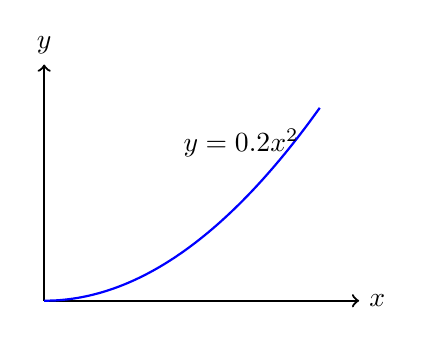
\begin{tikzpicture}
        \draw[thick, ->] (0,0) -- (4,0) node[right] {$x$};
        \draw[thick, ->] (0,0) -- (0,3) node[above] {$y$};
        \draw[blue, thick, domain=0:3.5, smooth, variable=\x] plot ({\x}, {0.2*\x*\x});
        \node at (2.5, 2) {$y = 0.2x^2$};
    \end{tikzpicture}
    \caption{A simple plot drawn with TikZ}
    \label{fig:tikzplot}
\end{figure}


% =============================================================================
%  CHAPTER 7: Cross References & Hyperlinks
% =============================================================================
% =============================================================================
%  CHAPTER 7: Cross References & Hyperlinks
% =============================================================================

\chapter{Cross References \& Hyperlinks}

\section{Labels and References}

\latex{} provides a powerful cross-referencing system. Every numbered element can be labeled and referenced.

\begin{lstlisting}[language={[LaTeX]TeX}, caption=Label and reference]
% Step 1: Place a label after the numbered element
\section{Introduction}
\label{sec:intro}

\begin{equation}
    E = mc^2
    \label{eq:einstein}
\end{equation}

\begin{figure}[htbp]
    \caption{My figure}
    \label{fig:myfig}
\end{figure}

\begin{table}[htbp]
    \caption{My table}
    \label{tab:mytab}
\end{table}

% Step 2: Reference it in text
As discussed in Section~\ref{sec:intro}...
Equation~\ref{eq:einstein} shows...
See Figure~\ref{fig:myfig} and Table~\ref{tab:mytab}.
\end{lstlisting}

\subsection{Label Naming Conventions}

\begin{table}[H]
\centering
\begin{tabular}{lll}
\toprule
\textbf{Element} & \textbf{Prefix} & \textbf{Example} \\
\midrule
Chapter    & \texttt{ch:}  & \texttt{ch:intro} \\
Section    & \texttt{sec:} & \texttt{sec:methods} \\
Subsection & \texttt{ssec:} & \texttt{ssec:data} \\
Figure     & \texttt{fig:} & \texttt{fig:diagram} \\
Table      & \texttt{tab:} & \texttt{tab:results} \\
Equation   & \texttt{eq:}  & \texttt{eq:euler} \\
Listing    & \texttt{lst:} & \texttt{lst:python} \\
Item       & \texttt{itm:} & \texttt{itm:first} \\
\bottomrule
\end{tabular}
\caption{Recommended label prefixes}
\end{table}

\subsection{Pageref and Nameref}

\begin{lstlisting}[language={[LaTeX]TeX}, caption=Other reference commands]
% Reference the page number:
See page~\pageref{sec:intro}.

% Reference the title/name:
Section~\nameref{sec:intro} discusses...

% Reference both name and page with autoref (hyperref):
\autoref{sec:intro}  % Produces "Section 1"
\autoref{fig:myfig}  % Produces "Figure 1"
\autoref{eq:einstein}% Produces "Equation 1"
\end{lstlisting}

% ------------------------------------------------------------------
\section{Hyperlinks (hyperref package)}

\begin{lstlisting}[language={[LaTeX]TeX}, caption=Hyperlinks]
\usepackage{hyperref}

% URL links:
\url{https://www.latex-project.org/}
\href{https://www.latex-project.org/}{LaTeX Project}

% Email link:
\href{mailto:user@example.com}{user@example.com}

% File link:
\href{file:///path/to/file}{Open file}

% Internal link (jump to label):
\hyperref[sec:intro]{Go to Introduction}

% Configuration:
\hypersetup{
    colorlinks=true,       % Colored links (not boxed)
    linkcolor=blue,        % Internal link color
    filecolor=magenta,     % File link color
    urlcolor=cyan,         % URL color
    citecolor=green,       % Citation color
}
\end{lstlisting}

Examples:
\begin{itemize}
    \item URL: \url{https://www.latex-project.org/}
    \item Hyperlinked text: \href{https://www.overleaf.com/}{Overleaf --- Online LaTeX Editor}
\end{itemize}

% ------------------------------------------------------------------
\section{Table of Contents}

\begin{lstlisting}[language={[LaTeX]TeX}, caption=Table of contents]
% Basic table of contents:
\tableofcontents

% List of figures:
\listoffigures

% List of tables:
\listoftables

% Limit TOC depth:
\setcounter{tocdepth}{2}  % Show up to subsection

% Set sectioning number depth:
\setcounter{secnumdepth}{3}  % Number up to subsubsection

% Add unnumbered section to TOC:
\section*{Acknowledgments}
\addcontentsline{toc}{section}{Acknowledgments}
\end{lstlisting}

\subsection{Custom TOC Entry}

\begin{lstlisting}[language={[LaTeX]TeX}, caption=Custom TOC entries]
% Add arbitrary entries to TOC:
\addcontentsline{toc}{chapter}{Preface}

% For the list of figures/tables:
\addcontentsline{lof}{figure}{My Figure Title}
\end{lstlisting}


% =============================================================================
%  CHAPTER 8: Bibliography
% =============================================================================
% =============================================================================
%  CHAPTER 8: Bibliography & Citations
% =============================================================================

\chapter{Bibliography \& Citations}

\section{Basic Bibliography with thebibliography}

The simplest way to create a bibliography is using the \texttt{thebibliography} environment directly.

\begin{lstlisting}[language={[LaTeX]TeX}, caption=thebibliography environment]
% At the end of your document (before \end{document}):
\begin{thebibliography}{9}
    \bibitem{knuth1984}
        Donald E. Knuth,
        \textit{The TeXbook},
        Addison-Wesley, 1984.

    \bibitem{lamport1994}
        Leslie Lamport,
        \textit{LaTeX: A Document Preparation System},
        Addison-Wesley, 2nd edition, 1994.

    \bibitem{mittelbach2004}
        Frank Mittelbach and Michel Goossens,
        \textit{The LaTeX Companion},
        Addison-Wesley, 2nd edition, 2004.
\end{thebibliography}

% Cite in text:
Knuth wrote the original TeX system~\cite{knuth1984}.
LaTeX was created by Lamport~\cite{lamport1994}.
\end{lstlisting}

\subsection{Citation Commands}

\begin{table}[H]
\centering
\begin{tabular}{lll}
\toprule
\textbf{Command} & \textbf{Output} & \textbf{Description} \\
\midrule
\verb|\cite{key}|         & [1]          & Basic citation \\
\verb|\cite[p.42]{key}|   & [1, p.42]    & With page number \\
\verb|\cite{a,b,c}|       & [1,2,3]      & Multiple citations \\
\bottomrule
\end{tabular}
\caption{Basic citation commands}
\end{table}

% ------------------------------------------------------------------
\section{BibTeX with .bib Files}

For larger projects, use a \texttt{.bib} file to manage references.

\subsection{The .bib File}

\begin{lstlisting}[caption=Sample .bib file (references.bib)]
@article{einstein1905,
    author  = {Albert Einstein},
    title   = {On the Electrodynamics of Moving Bodies},
    journal = {Annalen der Physik},
    year    = {1905},
    volume  = {322},
    number  = {10},
    pages   = {891--921},
    doi     = {10.1002/andp.19053221004}
}

@book{knuth1984,
    author    = {Donald E. Knuth},
    title     = {The TeXbook},
    publisher = {Addison-Wesley},
    year      = {1984},
    isbn      = {978-0201134483}
}

@inproceedings{lamport1998,
    author    = {Leslie Lamport},
    title     = {The Part-Time Parliament},
    booktitle = {ACM Transactions on Computer Systems},
    year      = {1998},
    volume    = {16},
    number    = {2},
    pages     = {133--169}
}

@online{overleaf2024,
    author  = {{Overleaf}},
    title   = {Documentation},
    year    = {2024},
    url     = {https://www.overleaf.com/learn}
}

@phdthesis{smith2020,
    author = {Jane Smith},
    title  = {Advanced Topics in Computer Science},
    school = {MIT},
    year   = {2020}
}
\end{lstlisting}

\subsection{Entry Types}

\begin{table}[H]
\centering
\begin{tabular}{ll}
\toprule
\textbf{Type} & \textbf{Used For} \\
\midrule
\texttt{@article}       & Journal articles \\
\texttt{@book}          & Books \\
\texttt{@booklet}       & Booklets / pamphlets \\
\texttt{@inbook}        & A chapter or section in a book \\
\texttt{@incollection}  & A chapter in a collected works \\
\texttt{@inproceedings} & Conference papers \\
\texttt{@manual}        & Technical documentation \\
\texttt{@mastersthesis} & Master's thesis \\
\texttt{@misc}          & Miscellaneous \\
\texttt{@phdthesis}     & PhD thesis \\
\texttt{@proceedings}   & Conference proceedings \\
\texttt{@techreport}    & Technical reports \\
\texttt{@unpublished}   & Unpublished works \\
\texttt{@online}        & Web resources \\
\bottomrule
\end{tabular}
\caption{BibTeX entry types}
\end{table}

\subsection{Common Fields}

\begin{table}[H]
\centering
\begin{tabular}{lll}
\toprule
\textbf{Field} & \textbf{Required} & \textbf{Description} \\
\midrule
\texttt{author}    & Most entries & Author names \\
\texttt{title}     & Most entries & Title of work \\
\texttt{year}      & Most entries & Year of publication \\
\texttt{publisher} & book, inbook & Publisher name \\
\texttt{journal}   & article      & Journal name \\
\texttt{volume}    & article      & Volume number \\
\texttt{number}    & article      & Issue number \\
\texttt{pages}     & article      & Page range \\
\texttt{doi}       & Optional     & Digital Object Identifier \\
\texttt{url}       & Optional     & URL to resource \\
\texttt{isbn}      & Optional     & ISBN number \\
\texttt{abstract}  & Optional     & Abstract text \\
\texttt{keywords}  & Optional     & Keywords \\
\bottomrule
\end{tabular}
\caption{Common BibTeX fields}
\end{table}

% ------------------------------------------------------------------
\section{Using BibTeX}

\begin{lstlisting}[language={[LaTeX]TeX}, caption=Using BibTeX]
% In your .tex file, at the end:
\bibliographystyle{plain}    % Choose a style
\bibliography{references}    % Name of .bib file (without .bib)

% Compilation steps:
% 1. pdflatex main.tex      (first pass)
% 2. bibtex main             (process citations)
% 3. pdflatex main.tex      (second pass)
% 4. pdflatex main.tex      (third pass for references)
\end{lstlisting}

\subsection{Bibliography Styles}

\begin{table}[H]
\centering
\begin{tabular}{ll}
\toprule
\textbf{Style} & \textbf{Description} \\
\midrule
\texttt{plain}    & Alphabetical by author, numbered [1] \\
\texttt{unsrt}    & Same as plain, but in order of citation \\
\texttt{alpha}    & Labels like [Knu84] (author-year abbrev.) \\
\texttt{abbrv}    & Like plain, with abbreviated first names \\
\texttt{ieeetr}   & IEEE Transactions style \\
\texttt{acm}      & ACM style \\
\texttt{apalike}  & APA-like style (author, year) \\
\bottomrule
\end{tabular}
\caption{Common bibliography styles}
\end{table}

% ------------------------------------------------------------------
\section{Biblatex (Modern Approach)}

\begin{lstlisting}[language={[LaTeX]TeX}, caption=biblatex package]
% In preamble:
\usepackage[backend=biber, style=numeric]{biblatex}
\addbibresource{references.bib}

% In document body:
As shown by~\textcite{einstein1905}...
According to~\autocite{knuth1984}...

% At end of document:
\printbibliography

% Or with a title:
\printbibliography[title={Works Cited}]

% Or filter by type:
\printbibliography[type=article, title={Journal Articles}]
\printbibliography[type=book, title={Books}]

% Citation commands unique to biblatex:
\cite{key}           % [1]
\parencite{key}      % (Author, Year)
\textcite{key}       % Author (Year)
\autocite{key}       % Depends on style
\footcite{key}       % Footnote citation
\end{lstlisting}

% ------------------------------------------------------------------
\section{Example Bibliography}

Here is a working example with inline references:

\begin{thebibliography}{9}
    \bibitem{knuth1984}
        Donald E. Knuth,
        \textit{The \TeX{}book},
        Addison-Wesley, 1984.

    \bibitem{lamport1994}
        Leslie Lamport,
        \textit{\LaTeX: A Document Preparation System},
        Addison-Wesley, 2nd edition, 1994.

    \bibitem{mittelbach2004}
        Frank Mittelbach and Michel Goossens,
        \textit{The \LaTeX{} Companion},
        Addison-Wesley, 2nd edition, 2004.

    \bibitem{overleaf2024}
        Overleaf,
        \textit{Learn \LaTeX{} in 30 Minutes},
        \url{https://www.overleaf.com/learn}, 2024.
\end{thebibliography}


% =============================================================================
%  CHAPTER 9: Code Listings & Verbatim
% =============================================================================
% =============================================================================
%  CHAPTER 9: Code Listings & Verbatim
% =============================================================================

\chapter{Code Listings \& Verbatim Text}

\section{Verbatim Text}

The \texttt{verbatim} environment prints text exactly as typed, without interpreting any \latex{} commands.

\begin{lstlisting}[language={[LaTeX]TeX}, caption=Verbatim environments]
% Inline verbatim:
\verb|This is \verbatim{test} text|

% Display verbatim:
\begin{verbatim}
    \textbf{This text is NOT bold}
    $E = mc^2$ is NOT an equation
    Everything appears exactly as typed!
\end{verbatim}

% Verbatim with different delimiter:
\verb!Special chars: $ % & # _ { }!

% With fancyvrb package (more options):
\usepackage{fancyvrb}
\begin{Verbatim}[fontsize=\small, frame=single, framesep=2mm]
    Custom verbatim with frame and smaller font
\end{Verbatim}
\end{lstlisting}

\subsection{Inline Verbatim Examples}

\begin{itemize}
    \item \verb|\documentclass{article}| — the document class command
    \item \verb|\usepackage{graphicx}| — loading a package
    \item \verb|$E = mc^2$| — inline math
\end{itemize}

% ------------------------------------------------------------------
\section{Code Listings (listings package)}

The \texttt{listings} package provides sophisticated source code formatting.

\subsection{Basic Listing}

\begin{lstlisting}[language=Python, caption=Basic code listing]
def hello_world():
    print("Hello, World!")
\end{lstlisting}

\subsection{Listing with Language}

\begin{lstlisting}[language=Python, caption=Python example with syntax highlighting]
# Python example: Fibonacci sequence
def fibonacci(n):
    """Calculate the nth Fibonacci number."""
    if n <= 1:
        return n
    a, b = 0, 1
    for _ in range(2, n + 1):
        a, b = b, a + b
    return b

# Generate first 10 Fibonacci numbers
for i in range(10):
    print(f"F({i}) = {fibonacci(i)}")
\end{lstlisting}

\subsection{Java Example}

\begin{lstlisting}[language=Java, caption=Java example]
public class HelloWorld {
    public static void main(String[] args) {
        System.out.println("Hello, World!");

        // Loop example
        for (int i = 0; i < 5; i++) {
            System.out.println("Iteration: " + i);
        }
    }
}
\end{lstlisting}

\subsection{C/C++ Example}

\begin{lstlisting}[language=C++, caption=C++ example]
#include <iostream>
#include <vector>
#include <algorithm>

int main() {
    std::vector<int> numbers = {5, 2, 8, 1, 9, 3};

    // Sort ascending
    std::sort(numbers.begin(), numbers.end());

    // Print sorted vector
    for (const auto& n : numbers) {
        std::cout << n << " ";
    }
    std::cout << std::endl;

    return 0;
}
\end{lstlisting}

\subsection{JavaScript Example}

\begin{lstlisting}[language=Java, caption=JavaScript example]
// Asynchronous data fetching
async function fetchData(url) {
    try {
        const response = await fetch(url);
        const data = await response.json();
        return data;
    } catch (error) {
        console.error("Error:", error);
    }
}
\end{lstlisting}

% ------------------------------------------------------------------
\section{Listing Styles and Configuration}

\begin{lstlisting}[language={[LaTeX]TeX}, caption=Listing configuration]
% Global settings in preamble:
\lstset{
    basicstyle=\ttfamily\small,          % Base font
    keywordstyle=\color{blue}\bfseries,  % Keywords
    commentstyle=\color{green!50!black}\itshape, % Comments
    stringstyle=\color{red!70!black},    % Strings
    numbers=left,                        % Line numbers
    numberstyle=\tiny\color{gray},       % Line number style
    stepnumber=1,                        % Line number step
    numbersep=5pt,                       % Distance of numbers
    backgroundcolor=\color{gray!5},      % Background color
    frame=single,                        % Border frame
    rulecolor=\color{gray!50},           % Frame color
    breaklines=true,                     % Auto line break
    breakatwhitespace=false,             % Break only at whitespace
    tabsize=4,                           % Tab size
    showstringspaces=false,              % Don't show string spaces
    captionpos=b,                        % Caption at bottom
    title=\lstname,                      % Show filename as title
}
\end{lstlisting}

\note{Per-listing options go in square brackets: \texttt{\textbackslash begin\{lstlisting\}[language=Python, caption=\{...\}]}.}

% ------------------------------------------------------------------
\section{Inline Code}

\begin{lstlisting}[language={[LaTeX]TeX}, caption=Inline code]
% Use \lstinline for inline code:
The function \lstinline|print("hello")| outputs text.

% Short form (define a shorthand):
\lstMakeShortInline[language=Python]{|}
Use |print("hello")| in your code.
\end{lstlisting}

% ------------------------------------------------------------------
\section{Supported Languages}

The listings package supports many programming languages:

\begin{table}[H]
\centering
\begin{tabular}{llll}
\toprule
\textbf{Language} & \textbf{Keyword} & \textbf{Language} & \textbf{Keyword} \\
\midrule
Python     & \texttt{Python}        & Java      & \texttt{Java} \\
C          & \texttt{C}             & C++       & \texttt{C++} \\
JavaScript & \texttt{Java}          & HTML      & \texttt{HTML} \\
SQL        & \texttt{SQL}           & R         & \texttt{R} \\
MATLAB     & \texttt{Matlab}        & Fortran   & \texttt{Fortran} \\
Bash       & \texttt{bash}          & XML       & \texttt{XML} \\
LaTeX      & \texttt{[LaTeX]TeX}    & Make      & \texttt{make} \\
\bottomrule
\end{tabular}
\caption{Some supported languages in the listings package}
\end{table}


% =============================================================================
%  CHAPTER 10: TikZ Graphics
% =============================================================================
% =============================================================================
%  CHAPTER 10: TikZ Graphics
% =============================================================================

\chapter{TikZ Graphics}

TikZ (``TikZ ist kein Zeichenprogramm'') is a powerful package for creating graphics directly in \latex{}.

\section{Basic Shapes}

\begin{figure}[H]
\centering
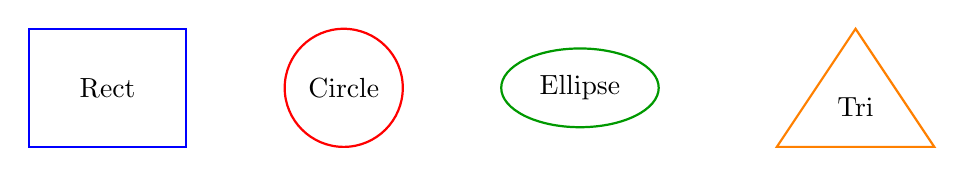
\begin{tikzpicture}
    % Rectangle
    \draw[thick, blue] (0,0) rectangle (2,1.5);
    \node at (1, 0.75) {Rect};

    % Circle
    \draw[thick, red] (4, 0.75) circle (0.75);
    \node at (4, 0.75) {Circle};

    % Ellipse
    \draw[thick, green!60!black] (7, 0.75) ellipse (1 and 0.5);
    \node at (7, 0.75) {Ellipse};

    % Triangle
    \draw[thick, orange] (9.5, 0) -- (11.5, 0) -- (10.5, 1.5) -- cycle;
    \node at (10.5, 0.5) {Tri};
\end{tikzpicture}
\caption{Basic shapes in TikZ}
\label{fig:tikzshapes}
\end{figure}

\begin{lstlisting}[language={[LaTeX]TeX}, caption=Basic shapes]
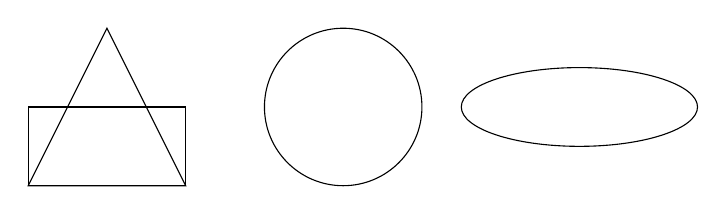
\begin{tikzpicture}
    \draw (0,0) rectangle (2,1);         % Rectangle
    \draw (4,1) circle (1);               % Circle
    \draw (7,1) ellipse (1.5 and 0.5);   % Ellipse
    \draw (0,0) -- (2,0) -- (1,2) -- cycle;  % Triangle
\end{tikzpicture}
\end{lstlisting}

% ------------------------------------------------------------------
\section{Lines and Paths}

\begin{figure}[H]
\centering
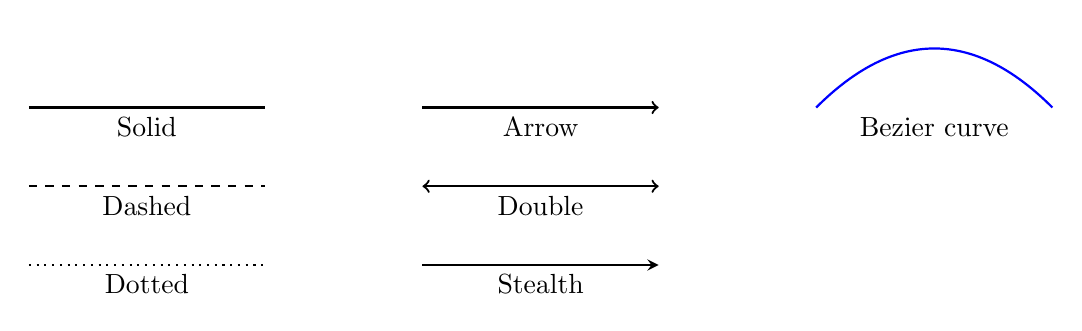
\begin{tikzpicture}
    % Solid line
    \draw[thick] (0,0) -- (3,0);
    \node[below] at (1.5,0) {Solid};

    % Dashed line
    \draw[thick, dashed] (0,-1) -- (3,-1);
    \node[below] at (1.5,-1) {Dashed};

    % Dotted line
    \draw[thick, dotted] (0,-2) -- (3,-2);
    \node[below] at (1.5,-2) {Dotted};

    % Arrow
    \draw[thick, ->] (5,0) -- (8,0);
    \node[below] at (6.5,0) {Arrow};

    % Double arrow
    \draw[thick, <->] (5,-1) -- (8,-1);
    \node[below] at (6.5,-1) {Double};

    % Stealth arrow
    \draw[thick, >=stealth, ->] (5,-2) -- (8,-2);
    \node[below] at (6.5,-2) {Stealth};

    % Curved path
    \draw[thick, blue] (10,0) .. controls (11,1) and (12,1) .. (13,0);
    \node[below] at (11.5,0) {Bezier curve};
\end{tikzpicture}
\caption{Lines and paths in TikZ}
\label{fig:tikzlines}
\end{figure}

% ------------------------------------------------------------------
\section{Filling and Colors}

\begin{figure}[H]
\centering
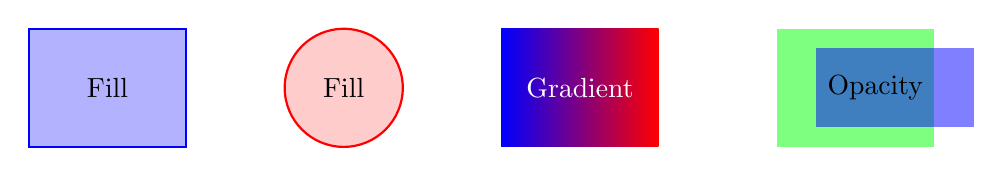
\begin{tikzpicture}
    % Filled shapes
    \fill[blue!30] (0,0) rectangle (2,1.5);
    \draw[blue, thick] (0,0) rectangle (2,1.5);
    \node at (1, 0.75) {Fill};

    \filldraw[fill=red!20, draw=red, thick] (4, 0.75) circle (0.75);
    \node at (4, 0.75) {Fill};

    % Gradient
    \shade[left color=blue, right color=red] (6,0) rectangle (8,1.5);
    \node[white] at (7, 0.75) {Gradient};

    % Opacity
    \fill[green, opacity=0.5] (9.5,0) rectangle (11.5,1.5);
    \fill[blue, opacity=0.5] (10,0.25) rectangle (12,1.25);
    \node at (10.75, 0.75) {Opacity};
\end{tikzpicture}
\caption{Filling and colors in TikZ}
\label{fig:tikzfill}
\end{figure}

% ------------------------------------------------------------------
\section{Nodes and Labels}

\begin{figure}[H]
\centering
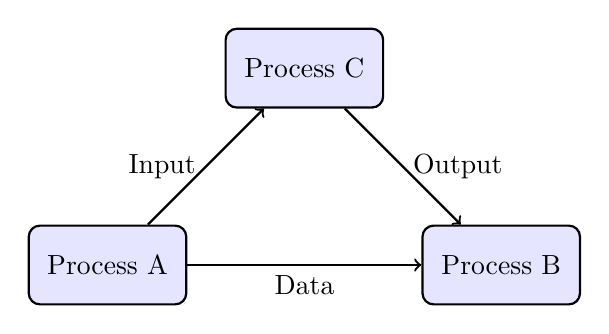
\begin{tikzpicture}[
    box/.style={rectangle, draw, thick, minimum width=2cm, minimum height=1cm,
                fill=blue!10, rounded corners, align=center},
    circle node/.style={circle, draw, thick, fill=red!10, minimum size=1cm}
]
    \node[box] (a) at (0,0) {Process A};
    \node[box] (b) at (5,0) {Process B};
    \node[box] (c) at (2.5,2.5) {Process C};

    \draw[->, thick] (a) -- (b) node[midway, below] {Data};
    \draw[->, thick] (a) -- (c) node[midway, left] {Input};
    \draw[->, thick] (c) -- (b) node[midway, right] {Output};
\end{tikzpicture}
\caption{Nodes and connections in TikZ}
\label{fig:tikznodes}
\end{figure}

\begin{lstlisting}[language={[LaTeX]TeX}, caption=Nodes and edges]
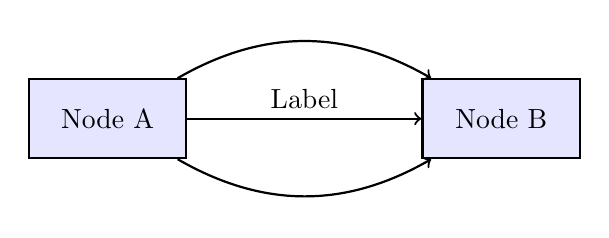
\begin{tikzpicture}[
    box/.style={rectangle, draw, thick, fill=blue!10,
                minimum width=2cm, minimum height=1cm}
]
    \node[box] (a) at (0,0) {Node A};
    \node[box] (b) at (5,0) {Node B};

    \draw[->, thick] (a) -- (b) node[midway, above] {Label};
    \draw[->, thick, bend left=30] (a) to (b);
    \draw[->, thick, bend right=30] (a) to[bend right] (b);
\end{tikzpicture}
\end{lstlisting}

% ------------------------------------------------------------------
\section{Flowchart}

% Uses the shapes.geometric library (for diamond) and positioning library
% (for below=of syntax). Both loaded in main.tex preamble.

\begin{figure}[H]
\centering
\begin{tikzpicture}[
    % Define reusable styles — these are just key-value defaults
    startstop/.style={rectangle, rounded corners, minimum width=3cm, minimum height=0.8cm,
                      text centered, draw=black, fill=red!20},
    process/.style={rectangle, minimum width=3cm, minimum height=0.8cm,
                    text centered, draw=black, fill=blue!15},
    decision/.style={diamond, aspect=2, minimum width=2.5cm,
                     text centered, draw=black, fill=green!15},
    arrow/.style={thick, -Stealth}   % -Stealth uses arrows.meta library
]
    \node (start)    [startstop]                    {Start};
    \node (input)    [process,  below=1cm of start] {Read Input};
    \node (decision) [decision, below=1cm of input] {Valid?};
    \node (process1) [process,  below=1cm of decision] {Process Data};
    \node (output)   [process,  right=3cm of decision] {Show Error};
    \node (stop)     [startstop, below=1cm of process1] {Stop};

    \draw [arrow] (start)    -- (input);
    \draw [arrow] (input)    -- (decision);
    \draw [arrow] (decision) -- node[left]  {Yes} (process1);
    \draw [arrow] (decision) -- node[above] {No}  (output);
    \draw [arrow] (output)   |- (input);
    \draw [arrow] (process1) -- (stop);
\end{tikzpicture}
\caption{Flowchart using TikZ (requires \texttt{shapes.geometric} and \texttt{positioning} libraries)}
\label{fig:flowchart}
\end{figure}

% ------------------------------------------------------------------
\section{Plots with pgfplots}

\begin{figure}[H]
\centering
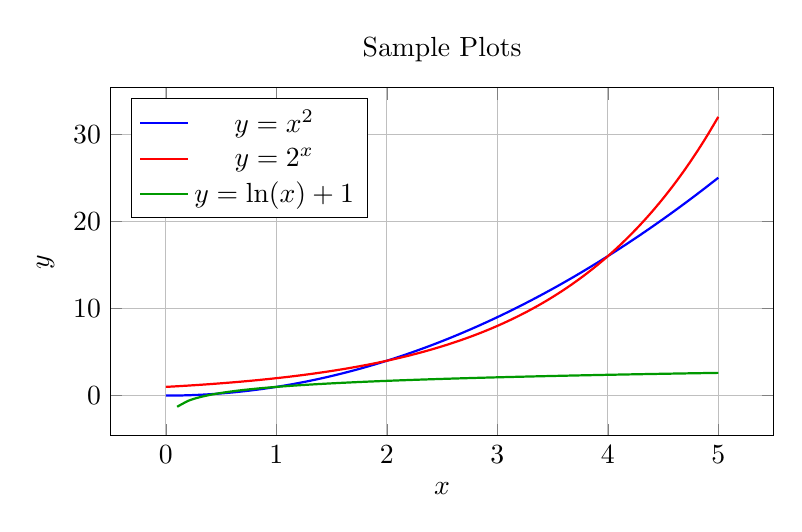
\begin{tikzpicture}
    \begin{axis}[
        xlabel={$x$},
        ylabel={$y$},
        title={Sample Plots},
        legend pos=north west,
        grid=major,
        width=10cm,
        height=6cm,
    ]
        \addplot[blue, thick, smooth, domain=0:5, samples=50] {x^2};
        \addlegendentry{$y = x^2$}

        \addplot[red, thick, smooth, domain=0:5, samples=50] {2^x};
        \addlegendentry{$y = 2^x$}

        \addplot[green!60!black, thick, smooth, domain=0:5, samples=50] {ln(x)+1};
        \addlegendentry{$y = \ln(x) + 1$}
    \end{axis}
\end{tikzpicture}
\caption{Function plots using pgfplots}
\label{fig:pgfplots}
\end{figure}

\begin{lstlisting}[language={[LaTeX]TeX}, caption=pgfplots example]
\usepackage{pgfplots}
\pgfplotsset{compat=1.18}

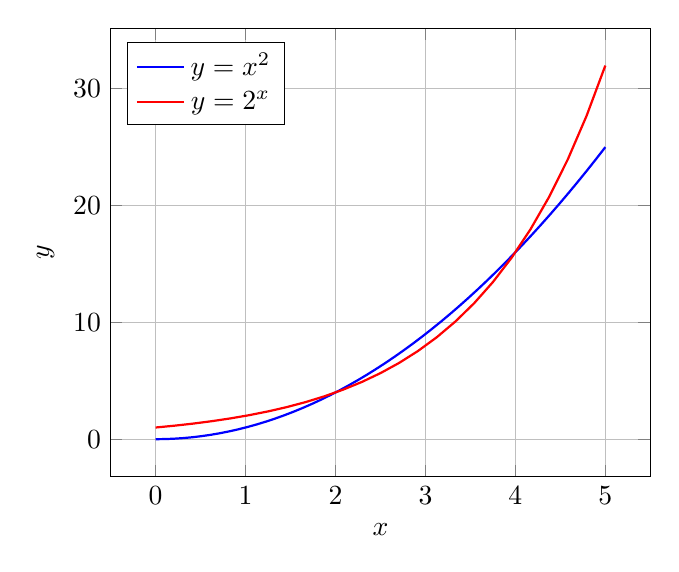
\begin{tikzpicture}
    \begin{axis}[
        xlabel={$x$}, ylabel={$y$},
        legend pos=north west,
        grid=major,
    ]
        \addplot[blue, thick, domain=0:5, samples=50] {x^2};
        \addlegendentry{$y = x^2$}

        \addplot[red, thick, domain=0:5] {2^x};
        \addlegendentry{$y = 2^x$}
    \end{axis}
\end{tikzpicture}
\end{lstlisting}

% ------------------------------------------------------------------
\section{Bar Chart}

\begin{figure}[H]
\centering
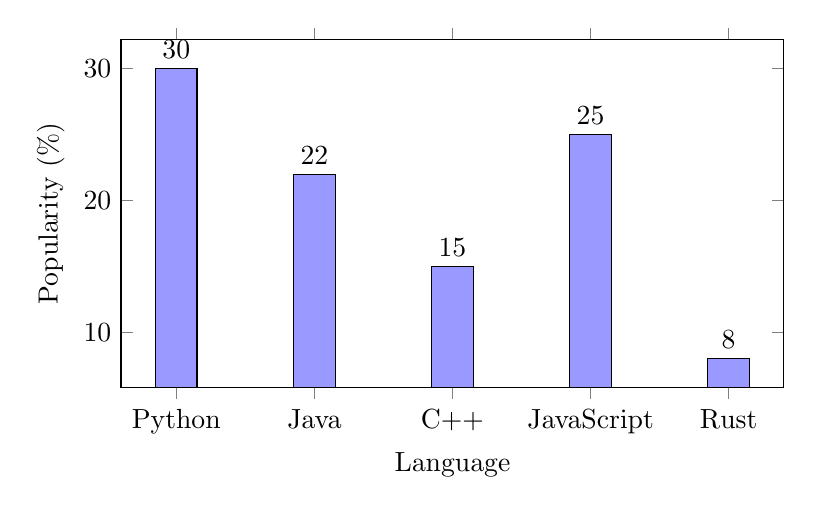
\begin{tikzpicture}
    \begin{axis}[
        ybar,
        xlabel={Language},
        ylabel={Popularity (\%)},
        symbolic x coords={Python, Java, C++, JavaScript, Rust},
        xtick=data,
        nodes near coords,
        nodes near coords align={vertical},
        width=10cm,
        height=6cm,
        bar width=15pt,
    ]
        \addplot[fill=blue!40] coordinates {
            (Python, 30) (Java, 22) (C++, 15) (JavaScript, 25) (Rust, 8)
        };
    \end{axis}
\end{tikzpicture}
\caption{Bar chart using pgfplots}
\label{fig:barchart}
\end{figure}

% ------------------------------------------------------------------
\section{TikZ Styles}

\begin{lstlisting}[language={[LaTeX]TeX}, caption=TikZ styles]
% Define reusable styles:
\tikzset{
    mybox/.style={
        rectangle, draw, thick,
        fill=blue!10,
        minimum width=2cm,
        minimum height=1cm,
        rounded corners=3pt,
        font=\sffamily
    },
    myarrow/.style={
        ->, >=stealth, thick, shorten >=1pt
    },
}

% Use them:
\node[mybox] (a) at (0,0) {Styled};
\node[mybox, fill=red!10] (b) at (3,0) {Override};
\draw[myarrow] (a) -- (b);
\end{lstlisting}


% =============================================================================
%  CHAPTER 11: Page Layout & Headers/Footers
% =============================================================================
% =============================================================================
%  CHAPTER 11: Page Layout & Headers/Footers
% =============================================================================

\chapter{Page Layout \& Headers/Footers}

\section{Page Geometry (geometry package)}

\begin{lstlisting}[language={[LaTeX]TeX}, caption=Page layout]
\usepackage{geometry}

% Set all margins at once:
\geometry{margin=2.5cm}

% Set individual margins:
\geometry{
    left=3cm,
    right=3cm,
    top=2cm,
    bottom=2cm,
    bindingoffset=5mm   % Extra for binding
}

% Landscape orientation:
\geometry{landscape}

% Paper size:
\geometry{a4paper}     % or letterpaper, legalpaper, a5paper
\end{lstlisting}

\subsection{Understanding Page Layout}

\begin{figure}[H]
\centering
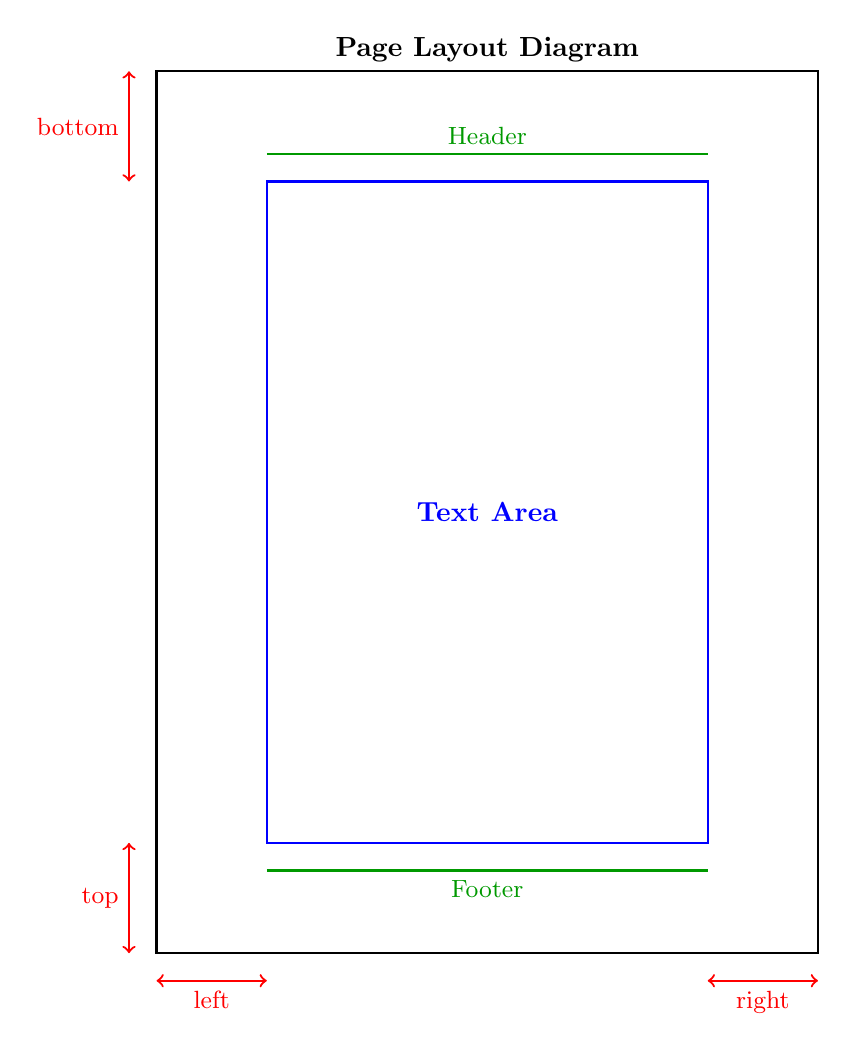
\begin{tikzpicture}[scale=0.7]
    % Page outline
    \draw[thick] (0,0) rectangle (12,16);
    \node[above] at (6,16) {\textbf{Page Layout Diagram}};

    % Text area
    \draw[blue, thick] (2,2) rectangle (10,14);
    \node[blue] at (6,8) {\textbf{Text Area}};

    % Margin labels
    \draw[<->, red, thick] (0,-0.5) -- (2,-0.5) node[midway, below] {\small left};
    \draw[<->, red, thick] (10,-0.5) -- (12,-0.5) node[midway, below] {\small right};
    \draw[<->, red, thick] (-0.5,0) -- (-0.5,2) node[midway, left] {\small top};
    \draw[<->, red, thick] (-0.5,14) -- (-0.5,16) node[midway, left] {\small bottom};

    % Header
    \draw[green!60!black, thick] (2,14.5) -- (10,14.5);
    \node[green!60!black, above] at (6,14.5) {\small Header};

    % Footer
    \draw[green!60!black, thick] (2,1.5) -- (10,1.5);
    \node[green!60!black, below] at (6,1.5) {\small Footer};
\end{tikzpicture}
\caption{Page layout anatomy}
\label{fig:pagelayout}
\end{figure}

% ------------------------------------------------------------------
\section{Headers and Footers (fancyhdr)}

\begin{lstlisting}[language={[LaTeX]TeX}, caption=fancyhdr package]
\usepackage{fancyhdr}
\pagestyle{fancy}

% Clear all defaults:
\fancyhf{}

% Set header:
\fancyhead[L]{Left header}       % L = Left
\fancyhead[C]{Center header}     % C = Center
\fancyhead[R]{Right header}      % R = Right

% Set footer:
\fancyfoot[L]{Author Name}
\fancyfoot[C]{\thepage}          % Page number
\fancyfoot[R]{\today}

% For even/odd pages (twoside):
\fancyhead[LE,RO]{\thepage}      % Left Even, Right Odd
\fancyhead[RE,LO]{\leftmark}     % Right Even, Left Odd

% Rule thickness:
\renewcommand{\headrulewidth}{0.4pt}
\renewcommand{\footrulewidth}{0pt}  % No footer rule

% Chapter page style (plain):
\fancypagestyle{plain}{
    \fancyhf{}
    \fancyfoot[C]{\thepage}
    \renewcommand{\headrulewidth}{0pt}
}
\end{lstlisting}

\subsection{Position Codes}

\begin{table}[H]
\centering
\begin{tabular}{ll}
\toprule
\textbf{Code} & \textbf{Position} \\
\midrule
\texttt{L} & Left \\
\texttt{C} & Center \\
\texttt{R} & Right \\
\texttt{E} & Even page \\
\texttt{O} & Odd page \\
\texttt{LE} & Left on even page \\
\texttt{RO} & Right on odd page \\
\bottomrule
\end{tabular}
\caption{Header/footer position codes}
\end{table}

% ------------------------------------------------------------------
\section{Page Numbering}

\begin{lstlisting}[language={[LaTeX]TeX}, caption=Page numbering]
% Numbering styles:
\pagenumbering{arabic}   % 1, 2, 3 (default)
\pagenumbering{roman}    % i, ii, iii
\pagenumbering{Roman}    % I, II, III
\pagenumbering{alph}     % a, b, c
\pagenumbering{Alph}     % A, B, C

% Set page counter:
\setcounter{page}{1}     % Start counting from 1

% No page number on current page:
\thispagestyle{empty}
\end{lstlisting}

% ------------------------------------------------------------------
\section{Multiple Columns}

\begin{lstlisting}[language={[LaTeX]TeX}, caption=Multiple columns]
% Document-wide twocolumn option:
\documentclass[twocolumn]{article}

% Switch mid-document:
\onecolumn   % Switch to one column
\twocolumn   % Switch to two columns

% With multicol package (more flexible):
\usepackage{multicol}

\begin{multicols}{3}  % 3 columns
    Text in column one continues into
    column two and then column three.
\end{multicols}

\begin{multicols}{2}[Section Title]
    Two-column section with a title.
\end{multicols}
\end{lstlisting}

% ------------------------------------------------------------------
\section{Page Breaks}

\begin{lstlisting}[language={[LaTeX]TeX}, caption=Page breaks]
\newpage         % Start a new page
\clearpage       % Flush all floats, then new page
\cleardoublepage % For twoside: go to next odd-numbered page
\pagebreak       % Suggest a page break (stretchable)
\nopagebreak     % Suggest no page break
\linebreak       % Suggest a line break
\nolinebreak     % Suggest no line break
\end{lstlisting}

% ------------------------------------------------------------------
\section{Paragraph Control}

\begin{lstlisting}[language={[LaTeX]TeX}, caption=Paragraph control]
% Paragraph indent:
\setlength{\parindent}{1cm}         % Set indent width
\noindent                           % No indent for this paragraph
\indent                             % Force indent

% Paragraph skip (no indent, vertical space instead):
\usepackage{parskip}               % Removes indent, adds space

% Or manually:
\setlength{\parindent}{0pt}
\setlength{\parskip}{6pt plus 2pt minus 1pt}
\end{lstlisting}


% =============================================================================
%  CHAPTER 12: Floating Bodies & Captions
% =============================================================================
% =============================================================================
%  CHAPTER 12: Floating Bodies & Captions
% =============================================================================

\chapter{Floating Bodies \& Captions}

\section{What Are Floats?}

Floats are objects (figures, tables) that \latex{} places at optimal positions in the document, rather than exactly where they appear in the source code.

\begin{table}[H]
\centering
\begin{tabular}{ll}
\toprule
\textbf{Environment} & \textbf{Content} \\
\midrule
\texttt{figure}   & Images, diagrams \\
\texttt{table}    & Tables \\
\texttt{algorithm} & Algorithms (with algorithm package) \\
\texttt{listing}  & Code listings (with listings package) \\
\bottomrule
\end{tabular}
\caption{Float environments}
\end{table}

% ------------------------------------------------------------------
\section{Placement Specifiers}

\begin{table}[H]
\centering
\begin{tabular}{llp{8cm}}
\toprule
\textbf{Specifier} & \textbf{Meaning} & \textbf{Notes} \\
\midrule
\texttt{h} & Here       & Approximately at the current location \\
\texttt{t} & Top        & At the top of the page \\
\texttt{b} & Bottom     & At the bottom of the page \\
\texttt{p} & Page       & On a separate float page \\
\texttt{!} & Override   & Override LaTeX's internal placement rules \\
\texttt{H} & HERE       & Exactly here (requires \texttt{float} package) \\
\bottomrule
\end{tabular}
\caption{Float placement specifiers}
\end{table}

\begin{lstlisting}[language={[LaTeX]TeX}, caption=Float placement]
\begin{figure}[htbp]     % Try here, top, bottom, then page
    ...
\end{figure}

\begin{figure}[H]        % Exactly here (float package)
    ...
\end{figure}

\begin{table}[!ht]       % Override rules, try here then top
    ...
\end{table}
\end{lstlisting}

% ------------------------------------------------------------------
\section{Captions}

\begin{lstlisting}[language={[LaTeX]TeX}, caption=Captions]
% Caption below the content (typical for figures):
\begin{figure}[htbp]
    \centering
    \includegraphics[width=5cm]{image}
    \caption{This is a figure caption.}
    \label{fig:myfigure}
\end{figure}

% Caption above the content (typical for tables):
\begin{table}[htbp]
    \centering
    \caption{This is a table caption.}
    \label{tab:mytable}
    \begin{tabular}{lc}
        ...
    \end{tabular}
\end{table}
\end{lstlisting}

\subsection{Caption Styles (caption package)}

\begin{lstlisting}[language={[LaTeX]TeX}, caption=Caption customization]
\usepackage{caption}

% Change label separator:
\captionsetup{labelsep=period}   % Figure 1. Caption text
\captionsetup{labelsep=quad}     % Figure 1    Caption text
\captionsetup{labelsep=newline}  % Label on separate line
\captionsetup{labelsep=none}     % No label

% Font options:
\captionsetup{font=small}
\captionsetup{font=it}
\captionsetup{labelfont=bf}

% Justification:
\captionsetup{justification=centering}
\captionsetup{justification=raggedright}
\captionsetup{justification=justified}

% Per-environment:
\captionsetup[figure]{font=small, labelfont=bf}
\captionsetup[table]{font=small, skip=5pt}
\end{lstlisting}

% ------------------------------------------------------------------
\section{Side Captions}

\begin{lstlisting}[language={[LaTeX]TeX}, caption=Side captions]
\usepackage{sidecap}

\begin{SCfigure}
    \includegraphics[width=5cm]{image}
    \caption{Caption appears beside the figure.}
\end{SCfigure}
\end{lstlisting}

% ------------------------------------------------------------------
\section{Float Barriers}

Sometimes floats drift too far from their reference. Use barriers to control this:

\begin{lstlisting}[language={[LaTeX]TeX}, caption=Float barriers]
\usepackage{placeins}

% Force all pending floats to be placed before this point:
\FloatBarrier

% Use in a section command:
\makeatletter
\AtBeginSection{\FloatBarrier}
\makeatother
\end{lstlisting}

% ------------------------------------------------------------------
\section{Controlling Float Counters}

\begin{lstlisting}[language={[LaTeX]TeX}, caption=Float counters]
% Maximum floats per page:
\renewcommand{\topfraction}{0.9}     % Max fraction of page for top floats
\renewcommand{\bottomfraction}{0.9}  % Max fraction for bottom floats
\renewcommand{\textfraction}{0.05}   % Min fraction for text
\renewcommand{\floatpagefraction}{0.8} % Min fraction of floats for float page

% Maximum number of floats:
\setcounter{topnumber}{4}            % Max top floats per page
\setcounter{bottomnumber}{4}         % Max bottom floats per page
\setcounter{totalnumber}{10}         % Max total floats per page
\end{lstlisting}


% =============================================================================
%  CHAPTER 13: Packages & Their Uses
% =============================================================================
% =============================================================================
%  CHAPTER 13: Essential Packages & Their Uses
% =============================================================================

\chapter{Essential Packages \& Their Uses}

\section{Package Management}

\begin{lstlisting}[language={[LaTeX]TeX}, caption=Loading packages]
% Basic syntax:
\usepackage{packagename}

% With options:
\usepackage[option1, option2]{packagename}

% Multiple packages at once:
\usepackage{package1, package2, package3}
\end{lstlisting}

\note{Packages must be loaded in the preamble (before \texttt{\textbackslash begin\{document\}}). Load \texttt{hyperref} last (or near-last) as a general rule.}

% ------------------------------------------------------------------
\section{Essential Package Reference}

\begin{longtable}{lp{4cm}p{6cm}}
\toprule
\textbf{Package} & \textbf{Category} & \textbf{Purpose} \\
\midrule
\endhead
\bottomrule
\endlastfoot

\texttt{inputenc}  & Encoding   & UTF-8 input encoding \\
\texttt{fontenc}   & Encoding   & Font encoding (T1) \\
\texttt{geometry}  & Layout     & Page margins and layout \\
\texttt{graphicx}  & Graphics   & Include images \\
\texttt{amsmath}   & Math       & Advanced math typesetting \\
\texttt{amssymb}   & Math       & Additional math symbols \\
\texttt{amsthm}    & Math       & Theorem environments \\
\texttt{booktabs}  & Tables     & Professional table rules \\
\texttt{array}     & Tables     & Extended column types \\
\texttt{tabularx}  & Tables     & Flexible-width tables \\
\texttt{longtable} & Tables     & Multi-page tables \\
\texttt{multirow}  & Tables     & Multi-row cells \\
\texttt{hyperref}  & Links      & Hyperlinks and cross-refs \\
\texttt{xcolor}    & Color      & Color support \\
\texttt{listings}  & Code       & Source code formatting \\
\texttt{tikz}      & Graphics   & Programmable drawings \\
\texttt{pgfplots}  & Graphics   & Plots and charts \\
\texttt{fancyhdr}  & Layout     & Headers and footers \\
\texttt{caption}   & Floats     & Caption customization \\
\texttt{subcaption}& Floats     & Subfigures/subtables \\
\texttt{enumitem}  & Lists      & Custom list formatting \\
\texttt{parskip}   & Layout     & Paragraph spacing \\
\texttt{float}     & Floats     & Improved float placement \\
\texttt{siunitx}   & Science    & SI units and numbers \\
\texttt{url}       & Links      & URL line breaking \\
\texttt{fancyvrb}  & Verbatim   & Enhanced verbatim \\
\texttt{multicol}  & Layout     & Multiple columns \\
\texttt{wrapfig}   & Floats     & Text-wrapped figures \\
\texttt{natbib}    & Bibliography & Flexible citations \\
\texttt{biblatex}  & Bibliography & Modern bibliography \\
\texttt{glossaries}& Reference  & Glossary / acronyms \\
\texttt{index}     & Reference  & Index generation \\
\texttt{nomencl}   & Reference  & Nomenclature lists \\
\texttt{appendix}  & Structure  & Appendix formatting \\
\texttt{titlesec}  & Structure  & Section title formatting \\
\texttt{tocloft}   & TOC        & TOC customization \\
\texttt{setspace}  & Layout     & Line spacing control \\
\texttt{ulem}      & Text       & Underline / strikethrough \\
\texttt{textcomp}  & Symbols    & Additional text symbols \\
\texttt{placeins}  & Floats     & Float barriers \\
\end{longtable}

% ------------------------------------------------------------------
\section{Package Conflicts and Loading Order}

\begin{lstlisting}[language={[LaTeX]TeX}, caption=Recommended loading order]
% 1. Encoding
\usepackage[utf8]{inputenc}
\usepackage[T1]{fontenc}

% 2. Language (babel or polyglossia)
\usepackage[english]{babel}

% 3. Fonts
\usepackage{lmodern}   % Latin Modern fonts

% 4. Math
\usepackage{amsmath, amssymb, amsthm}

% 5. Graphics and drawing
\usepackage{graphicx}
\usepackage{tikz}

% 6. Tables
\usepackage{booktabs, array, tabularx}

% 7. Layout
\usepackage{geometry}
\usepackage{fancyhdr}

% 8. Lists and text
\usepackage{enumitem}
\usepackage{xcolor}

% 9. Code
\usepackage{listings}

% 10. Bibliography
\usepackage{natbib}  % or biblatex

% 11. Hyperref (ALWAYS LAST or near-last)
\usepackage{hyperref}

% 12. Appendix (after hyperref)
\usepackage{appendix}
\end{lstlisting}

% ------------------------------------------------------------------
\section{SI Units (siunitx)}

\begin{lstlisting}[language={[LaTeX]TeX}, caption=siunitx package]
\usepackage{siunitx}

% Number formatting:
\num{12345.67}              % 12 345.67
\num{1.23e4}                % 1.23 x 10^4
\num[round-precision=2]{3.14159}  % 3.14

% Units:
\si{kg}                     % kg
\si{m/s}                    % m/s
\si{kg.m.s^{-2}}            % kg m s^-2
\si{\meter\per\second}      % m/s (symbolic)

% Value + unit:
\SI{9.8}{m/s^2}             % 9.8 m/s^2
\SI{100}{\degreeCelsius}    % 100 degrees C
\SI{3.14}{\micro\meter}     % 3.14 micrometer
\end{lstlisting}

Examples: The speed of light is \SI{3e8}{m/s}. Water boils at \SI{100}{\degreeCelsius}. The wavelength is \SI{550}{\nano\meter}.

% ------------------------------------------------------------------
\section{Creating Your Own Package}

\begin{lstlisting}[language={[LaTeX]TeX}, caption=Creating a package]
% Save as mystyle.sty:
\NeedsTeXFormat{LaTeX2e}
\ProvidesPackage{mystyle}[2024/01/01 My Custom Style]

% Package options:
\DeclareOption{draft}{\typeout{Draft mode}}
\ProcessOptions\relax

% Load required packages:
\RequirePackage{amsmath}
\RequirePackage{graphicx}

% Define commands:
\newcommand{\emphasis}[1]{\textbf{\textit{#1}}}

\endinput
% Then in your document:
% \usepackage{mystyle}
\end{lstlisting}


% =============================================================================
%  CHAPTER 14: Custom Commands & Environments
% =============================================================================
% =============================================================================
%  CHAPTER 14: Custom Commands & Environments
% =============================================================================

\chapter{Custom Commands \& Environments}

\section{New Commands (\texttt{\textbackslash newcommand})}

\begin{lstlisting}[language={[LaTeX]TeX}, caption=newcommand syntax]
% Basic: no arguments
\newcommand{\myname}{John Doe}
Hello, I am \myname.          % Output: Hello, I am John Doe.

% With arguments (1 required argument):
\newcommand{\greet}[1]{Hello, #1!}
\greet{Alice}                 % Output: Hello, Alice!

% With multiple arguments:
\newcommand{\add}[2]{#1 + #2}
$\add{a}{b}$                  % Output: a + b

% With optional arguments:
\newcommand{\hello}[2][World]{Hello, #2 from #1!}
\hello{Alice}                 % Output: Hello, Alice from World!
\hello[Bob]{Alice}            % Output: Hello, Alice from Bob!

% Maximum 9 arguments (#1 through #9)
\end{lstlisting}

\subsection{Practical Examples}

\begin{lstlisting}[language={[LaTeX]TeX}, caption=Practical custom commands]
% Shorthand for common formatting:
\newcommand{\pkg}[1]{\texttt{#1}}
\newcommand{\cmd}[1]{\texttt{\textbackslash#1}}

% Math shortcuts:
\newcommand{\R}{\mathbb{R}}              % Real numbers
\newcommand{\norm}[1]{\left\|#1\right\|} % Norm notation
\newcommand{\abs}[1]{\left|#1\right|}    % Absolute value
\newcommand{\inner}[2]{\langle #1, #2 \rangle} % Inner product
\newcommand{\dd}{\,\mathrm{d}}           % Differential d

% Usage:
% $f\colon \R^n \to \R$
% $\norm{x} = \sqrt{\inner{x}{x}}$
% $\int_0^1 f(x) \dd x$
\end{lstlisting}

Results:
\[ f\colon \mathbb{R}^n \to \mathbb{R}, \quad \|x\| = \sqrt{\langle x, x \rangle} \]

% ------------------------------------------------------------------
\section{Renaming Commands (\texttt{\textbackslash renewcommand})}

\begin{lstlisting}[language={[LaTeX]TeX}, caption=renewcommand]
% Override existing commands:
\renewcommand{\contentsname}{Contents}        % Rename TOC title
\renewcommand{\figurename}{Fig.}              % Rename figure label
\renewcommand{\tablename}{Table}              % Rename table label
\renewcommand{\bibname}{References}           % Rename bibliography

% Check if command exists:
\providecommand{\mycommand}{default value}   % Define only if not already
\end{lstlisting}

% ------------------------------------------------------------------
\section{New Environments}

You can define entire environments (begin/end pairs) with \verb|\newenvironment|:

The syntax is:
\verb|\newenvironment{name}[args]{begin-code}{end-code}|

\textbf{Example 1} -- a simple warning box:
\begin{lstlisting}[language={[LaTeX]TeX}]
\newenvironment{warning}
    {\begin{center}\bfseries Warning: }
    {\end{center}}
\end{lstlisting}

\textbf{Example 2} -- a box with a title argument:
\begin{lstlisting}[language={[LaTeX]TeX}]
\newenvironment{infobox}[1]
    {\begin{center}\fbox{\parbox{0.9\textwidth}%
     {\textbf{##1}\par\smallskip}}}
    {\end{center}}
\end{lstlisting}

% ------------------------------------------------------------------
\section{Lengths and Counters}

\subsection{Defining Lengths}

\begin{Verbatim}[frame=single, fontsize=\small, label=Custom lengths]
% Create a new length:
\newlength{\mywidth}
\setlength{\mywidth}{5cm}

% Use it:
\hspace{\mywidth}

% Arithmetic on lengths:
\addtolength{\mywidth}{2cm}           % Add 2cm
\settowidth{\mywidth}{Hello World}    % Set to width of text
\settoheight{\myheight}{Text}         % Set to height
\settodepth{\mydepth}{Text}           % Set to depth
\end{Verbatim}

\subsection{Standard Lengths}

\begin{table}[H]
\centering
\begin{tabular}{ll}
\toprule
\textbf{Length} & \textbf{Controls} \\
\midrule
\verb|\textwidth|      & Width of text area \\
\verb|\linewidth|      & Width of current line \\
\verb|\columnwidth|    & Width of column \\
\verb|\paperwidth|     & Width of paper \\
\verb|\paperheight|    & Height of paper \\
\verb|\parindent|      & Paragraph indentation \\
\verb|\parskip|        & Space between paragraphs \\
\verb|\baselineskip|   & Distance between baselines \\
\verb|\columnsep|      & Space between columns \\
\bottomrule
\end{tabular}
\caption{Standard \latex{} lengths}
\end{table}

\subsection{Counters}

\begin{lstlisting}[language={[LaTeX]TeX}, caption=Counters]
% Define a new counter:
\newcounter{mycounter}

% Set, step, and use:
\setcounter{mycounter}{0}
\stepcounter{mycounter}      % Increment by 1
\addtocounter{mycounter}{5}  % Add 5

% Display:
\arabic{mycounter}   % 1, 2, 3
\roman{mycounter}    % i, ii, iii
\Roman{mycounter}    % I, II, III
\alph{mycounter}     % a, b, c
\Alph{mycounter}     % A, B, C
\fnsymbol{mycounter} % *, dagger, double-dagger, etc.
\end{lstlisting}

% ------------------------------------------------------------------
\section{Conditional Commands}

\begin{lstlisting}[language={[LaTeX]TeX}, caption=Conditionals]
% ifthen package:
\usepackage{ifthen}

\newcommand{\checkodd}[1]{%
    \ifthenelse{\isodd{#1}}%
        {#1 is odd}%
        {#1 is even}%
}

% Boolean flags:
\newboolean{draftmode}
\setboolean{draftmode}{true}

\ifthenelse{\boolean{draftmode}}%
    {\watermark{DRAFT}}%
    {}
\end{lstlisting}

% ------------------------------------------------------------------
\section{Boxes}

\begin{Verbatim}[frame=single, fontsize=\small, label=Boxes]
% mbox: prevents line breaks
\mbox{This text stays on one line}

% fbox: framed box
\fbox{Framed text}

% makebox: custom box with alignment
\makebox[5cm][c]{Centered in 5cm}
% Alignment: l=left, c=center, r=right, s=stretch

% parbox: paragraph in a box
\parbox{3cm}{This text wraps inside a 3cm-wide box.}

% minipage: like parbox but more powerful
\begin{minipage}[t]{0.45\textwidth}
    Left column content.
\end{minipage}
\hfill
\begin{minipage}[t]{0.45\textwidth}
    Right column content.
\end{minipage}

% raisebox: vertically offset text
\raisebox{5pt}{Raised text}
\raisebox{-5pt}{Lowered text}
\end{Verbatim}

Side-by-side minipage example:

\begin{minipage}[t]{0.45\textwidth}
    \textbf{Left Column}\\
    This content sits in the left minipage. It wraps automatically within the specified width.
\end{minipage}%
\hfill
\begin{minipage}[t]{0.45\textwidth}
    \textbf{Right Column}\\
    This content sits in the right minipage. Using minipages we can create multi-column layouts anywhere.
\end{minipage}


% =============================================================================
%  CHAPTER 15: Advanced Topics
% =============================================================================
% =============================================================================
%  CHAPTER 15: Advanced Topics
% =============================================================================

\chapter{Advanced Topics}

\section{Tables of Contents for Non-Standard Sections}

\begin{lstlisting}[language={[LaTeX]TeX}, caption=Custom TOC entries]
% Add unnumbered chapter to TOC:
\chapter*{Preface}
\addcontentsline{toc}{chapter}{Preface}

% Custom TOC depth:
\setcounter{tocdepth}{2}     % Show sections and subsections only
\setcounter{secnumdepth}{3}  % Number up to subsubsection

% Mini table of contents per chapter (minitoc package):
\usepackage{minitoc}
\dominitoc                      % In preamble, after \tableofcontents
\chapter{My Chapter}
\minitoc                        % Shows TOC for this chapter only
\end{lstlisting}

% ------------------------------------------------------------------
\section{Index}

\begin{lstlisting}[language={[LaTeX]TeX}, caption=Index]
\usepackage{makeidx}
\makeindex                       % In preamble

% Mark entries:
\index{keyword}
\index{main topic!subtopic}     % Nested index entry
\index{term|textbf}             % Bold page reference

% Special characters:
\index{keyword@\texttt{keyword}}  % Custom sort vs display

% Print the index:
\printindex                      % At end of document

% Compilation:
% pdflatex main.tex
% makeindex main
% pdflatex main.tex
\end{lstlisting}

% ------------------------------------------------------------------
\section{Glossary / Acronyms}

\begin{lstlisting}[language={[LaTeX]TeX}, caption=Glossary]
\usepackage[acronym, toc]{glossaries}
\makeglossaries

% Define terms:
\newglossaryentry{latex}{
    name=LaTeX,
    description={A document preparation system}
}

\newacronym{api}{API}{Application Programming Interface}

% Use in text:
\gls{latex}         % First: "LaTeX (A document preparation system)"
                     % Later: "LaTeX"
\gls{api}           % First: "Application Programming Interface (API)"
                     % Later: "API"
\Gls{latex}         % Capitalized first letter

% Print glossary:
\printglossary[type=main]          % Glossary
\printglossary[type=\acronymtype]  % Acronyms
\end{lstlisting}

% ------------------------------------------------------------------
\section{Watermarks}

\begin{lstlisting}[language={[LaTeX]TeX}, caption=Watermark]
\usepackage[firstpage]{draftwatermark}
\SetWatermarkText{CONFIDENTIAL}
\SetWatermarkScale{3}
\SetWatermarkColor[gray]{0.9}
\SetWatermarkAngle{45}

% Or with wallpaper package for images:
\usepackage{wallpaper}
\ThisCenterWallPaper{0.5}{logo.png}
\end{lstlisting}

% ------------------------------------------------------------------
\section{Conditional Compilation}

\begin{lstlisting}[language={[LaTeX]TeX}, caption=Conditional compilation]
% Define a flag:
\newif\ifdraft
\drafttrue          % Set to draft mode
% \draftfalse       % Set to final mode

% Use conditionally:
\ifdraft
    \usepackage[draft]{graphicx}  % Show image boxes only
\else
    \usepackage{graphicx}         % Full images
\fi

% Include content conditionally:
\ifdraft
    \include{chapters/draft-notes}
\fi

% Version control:
\newcommand{\version}{1.0}
\newcommand{\releasedate}{2024-01-01}
\end{lstlisting}

% ------------------------------------------------------------------
\section{External Files and Shell Escape}

\begin{lstlisting}[language={[LaTeX]TeX}, caption=File operations]
% Read from external file:
\input{data/variables.tex}        % Insert file content

% Write to file (during compilation):
\newwrite\myoutput
\immediate\openout\myoutput=output.txt
\immediate\write\myoutput{Hello from LaTeX}
\immediate\closeout\myoutput

% Shell escape (compile with --shell-escape):
% \write18{date > date.txt}
% \input{date.txt}
\end{lstlisting}

% ------------------------------------------------------------------
\section{Compilation Tools}

\subsection{latexmk}

\begin{lstlisting}[caption=latexmk automation]
# latexmk automates multi-pass compilation:
latexmk -pdf main.tex              % Compile to PDF
latexmk -xelatex main.tex          % Use XeLaTeX
latexmk -lualatex main.tex         % Use LuaLaTeX
latexmk -c                         % Clean auxiliary files
latexmk -C                         % Clean all (including PDF)
latexmk -pvc main.tex              % Preview continuously (live reload)
\end{lstlisting}

\subsection{Compilation Engines}

\begin{table}[H]
\centering
\begin{tabular}{lll}
\toprule
\textbf{Engine} & \textbf{Command} & \textbf{Best For} \\
\midrule
pdfLaTeX  & \texttt{pdflatex}  & Standard documents, English \\
XeLaTeX   & \texttt{xelatex}   & Unicode, system fonts \\
LuaLaTeX  & \texttt{lualatex}  & Advanced scripting, Lua integration \\
\bottomrule
\end{tabular}
\caption{\latex{} compilation engines}
\end{table}

\subsection{Using System Fonts (XeLaTeX/LuaLaTeX)}

\begin{lstlisting}[caption=System fonts with fontspec]
% Requires XeLaTeX or LuaLaTeX
\usepackage{fontspec}

% Set main font:
\setmainfont{Times New Roman}
\setsansfont{Arial}
\setmonofont{Consolas}

% With options:
\setmainfont[
    BoldFont=Times New Roman Bold,
    ItalicFont=Times New Roman Italic,
    Scale=1.0
]{Times New Roman}
\end{lstlisting}

% ------------------------------------------------------------------
\section{Beamer Presentations (Overview)}

\begin{lstlisting}[language={[LaTeX]TeX}, caption=Beamer basics]
\documentclass{beamer}
\usetheme{Madrid}
\usecolortheme{default}

\title{My Presentation}
\author{Author Name}
\date{\today}

\begin{document}

\begin{frame}
    \titlepage
\end{frame}

\begin{frame}{Outline}
    \tableofcontents
\end{frame}

\begin{frame}{My First Slide}
    \begin{itemize}
        \item First point
        \item Second point
    \end{itemize}
\end{frame}

% Columns:
\begin{frame}{Two Columns}
    \begin{columns}
        \column{0.5\textwidth}
            Left content
        \column{0.5\textwidth}
            Right content
    \end{columns}
\end{frame}

% Overlays (step-by-step reveal):
\begin{frame}{Overlays}
    \begin{itemize}
        \item<1-> First (appears on slide 1+)
        \item<2-> Second (appears on slide 2+)
        \item<3-> Third (appears on slide 3+)
    \end{itemize}
\end{frame}
\end{document}
\end{lstlisting}

% ------------------------------------------------------------------
\section{Multilingual Support}

\begin{lstlisting}[language={[LaTeX]TeX}, caption=Multilingual documents]
% With babel:
\usepackage[english, french, german]{babel}
% Last language is default. Switch:
\selectlanguage{french}
\selectlanguage{english}

% With polyglossia (XeLaTeX/LuaLaTeX):
\usepackage{polyglossia}
\setdefaultlanguage{english}
\setotherlanguage{french}
\setotherlanguage{german}

\begin{german}
    Hallo Welt!
\end{german}
\end{lstlisting}

% ------------------------------------------------------------------
\section{Error Handling}

\begin{table}[H]
\centering
\begin{tabular}{lp{8cm}}
\toprule
\textbf{Error} & \textbf{Common Cause} \\
\midrule
\texttt{Undefined control sequence} & Misspelled command or missing package \\
\texttt{Missing \$ inserted}       & Used math symbol outside math mode \\
\texttt{Extra alignment tab}       & Too many \texttt{\&} in table row \\
\texttt{Missing \} inserted}       & Unmatched braces \\
\texttt{Float too large}           & Figure/table wider than text area \\
\texttt{Overfull \textbackslash hbox} & Text extends past margin \\
\texttt{Underfull \textbackslash hbox} & Too much whitespace in line \\
\bottomrule
\end{tabular}
\caption{Common \latex{} errors}
\end{table}

\note{Always read the \texttt{.log} file for detailed error information. The first error reported is usually the root cause.}


% --- APPENDIX ---
\appendix
% =============================================================================
%  APPENDIX
% =============================================================================

\chapter{Quick Reference Card}

\section{Document Skeleton}

\begin{lstlisting}[language={[LaTeX]TeX}, caption=Complete document skeleton]
\documentclass[12pt, a4paper]{report}

% === PREAMBLE ===
\usepackage[utf8]{inputenc}
\usepackage[T1]{fontenc}
\usepackage{geometry}
\usepackage{graphicx}
\usepackage{amsmath, amssymb}
\usepackage{booktabs}
\usepackage{hyperref}
\usepackage{xcolor}
\usepackage{listings}
\usepackage{tikz}

\title{My Document Title}
\author{Author Name}
\date{\today}

% === BODY ===
\begin{document}
\maketitle
\tableofcontents

\chapter{Introduction}
\label{ch:intro}

\section{Background}
\label{sec:background}

Text with \textbf{bold}, \textit{italic}, and \texttt{monospace}.

Inline math: $E = mc^2$

Display math:
\[ \int_0^\infty e^{-x^2} dx = \frac{\sqrt{\pi}}{2} \]

\begin{figure}[htbp]
    \centering
    \includegraphics[width=0.6\textwidth]{myimage}
    \caption{My figure.}
    \label{fig:myfigure}
\end{figure}

\begin{table}[htbp]
    \centering
    \caption{My table.}
    \label{tab:mytable}
    \begin{tabular}{lcc}
        \toprule
        Name & Value & Note \\
        \midrule
        A    & 1     & x \\
        B    & 2     & y \\
        \bottomrule
    \end{tabular}
\end{table}

\bibliographystyle{plain}
\bibliography{references}

\end{document}
\end{lstlisting}

% ------------------------------------------------------------------
\section{Symbol Quick Reference}

\begin{table}[H]
\centering
\begin{tabular}{llll}
\toprule
\textbf{Symbol} & \textbf{Code} & \textbf{Symbol} & \textbf{Code} \\
\midrule
$\alpha$   & \verb|\alpha|   & $\beta$    & \verb|\beta| \\
$\gamma$   & \verb|\gamma|   & $\delta$   & \verb|\delta| \\
$\epsilon$ & \verb|\epsilon| & $\theta$   & \verb|\theta| \\
$\lambda$  & \verb|\lambda|  & $\mu$      & \verb|\mu| \\
$\pi$      & \verb|\pi|      & $\sigma$   & \verb|\sigma| \\
$\phi$     & \verb|\phi|     & $\omega$   & \verb|\omega| \\
$\sum$     & \verb|\sum|     & $\prod$    & \verb|\prod| \\
$\int$     & \verb|\int|     & $\sqrt{x}$ & \verb|\sqrt{x}| \\
$\frac{a}{b}$ & \verb|\frac{a}{b}| & $\infty$ & \verb|\infty| \\
$\forall$  & \verb|\forall|  & $\exists$  & \verb|\exists| \\
$\in$      & \verb|\in|      & $\notin$   & \verb|\notin| \\
$\subset$  & \verb|\subset|  & $\cup$     & \verb|\cup| \\
$\cap$     & \verb|\cap|     & $\emptyset$& \verb|\emptyset| \\
$\to$      & \verb|\to|      & $\Rightarrow$ & \verb|\Rightarrow| \\
$\leq$     & \verb|\leq|     & $\geq$     & \verb|\geq| \\
$\neq$     & \verb|\neq|     & $\approx$  & \verb|\approx| \\
$\pm$      & \verb|\pm|      & $\times$   & \verb|\times| \\
$\cdot$    & \verb|\cdot|    & $\ldots$   & \verb|\ldots| \\
$\cdots$   & \verb|\cdots|   & $\vdots$   & \verb|\vdots| \\
\bottomrule
\end{tabular}
\caption{Common math symbols quick reference}
\end{table}

% ------------------------------------------------------------------
\section{Useful Commands Cheat Sheet}

\begin{table}[H]
\centering
\begin{tabular}{ll}
\toprule
\textbf{Command} & \textbf{Purpose} \\
\midrule
\verb|\documentclass{article}| & Set document type \\
\verb|\usepackage{pkg}|       & Load a package \\
\verb|\begin{env}...\end{env}| & Use an environment \\
\verb|\textbf{text}|          & Bold text \\
\verb|\textit{text}|          & Italic text \\
\verb|\texttt{text}|          & Monospace text \\
\verb|\underline{text}|       & Underlined text \\
\verb|\textcolor{red}{text}|  & Colored text \\
\verb|\footnote{text}|        & Footnote \\
\verb|\cite{key}|             & Citation \\
\verb|\ref{label}|            & Cross reference \\
\verb|\pageref{label}|        & Page reference \\
\verb|\label{key}|            & Define label \\
\verb|\includegraphics{file}| & Include image \\
\verb|\tableofcontents|       & Table of contents \\
\verb|\listoffigures|         & List of figures \\
\verb|\listoftables|          & List of tables \\
\verb|\appendix|              & Start appendix \\
\verb|\today|                 & Current date \\
\verb|\LaTeX|                 & LaTeX logo \\
\verb|\TeX|                   & TeX logo \\
\bottomrule
\end{tabular}
\caption{Essential commands cheat sheet}
\end{table}

% ------------------------------------------------------------------
\section{Compilation Workflow}

\begin{table}[H]
\centering
\begin{tabular}{ll}
\toprule
\textbf{Task} & \textbf{Commands} \\
\midrule
Basic compile  & \texttt{pdflatex main.tex} \\
With BibTeX    & \texttt{pdflatex main} $\to$ \texttt{bibtex main} $\to$ \texttt{pdflatex main} $\times 2$ \\
With glossary  & Add \texttt{makeglossaries main} after first compile \\
Automated      & \texttt{latexmk -pdf main.tex} \\
Clean aux      & \texttt{latexmk -c} \\
\bottomrule
\end{tabular}
\caption{Compilation workflows}
\end{table}


\end{document}
